\documentclass[11pt,a4paper,italian]{article}
\usepackage[utf8]{inputenc}
\usepackage{amsmath}
\usepackage{amsfonts}
\usepackage{amssymb}
\usepackage{graphicx} 
\usepackage{float}
\usepackage{verbatim}
\usepackage[italian]{babel}% per avere la scritta "Indice"
\usepackage{comment}

\begin{document}
\setcounter{section}{0}
\setcounter{page}{1}
%INDEX OF PAGES
\tableofcontents \pagebreak

\section{Analisi dei dati di probabilit\`a}
\label{Analisi dei dati}

Durante il periodo 20/05 - 24/05 mi sono occupata di analizzare la probabilit\`a che ha un candidato di rispondere correttamente alle domande in fase di test; valutando le relazioni di dipendenza che possono esistere tra pi\`u domande e l'impatto che pu\`o assumere la fortuna.

\subsection{Problema in esame}
\label{Problema in esame}

Test, sottoposto ad un candidato  durante un colloquio, composto da \textit{domande a tripla risposta multipla}.\\\\ Nel suddetta sezione vengono analizzate le relazioni che intercorrono tra due domande, denominate A e B, a seconda se il candidato risulta in grado di rispondervi correttamente o meno.

\subsection{Caratteristiche degli eventi di coppia}
\label{Caratteristiche degli eventi di coppia}

Tipi di eventi trattati:
\begin{itemize}
\item \textbf{Eventi indipendenti};
\item \textbf{Eventi dipendenti}:
  \begin{itemize}
  \item A e B sono strettamente dipendenti;
  \item A implica B.
  \end{itemize}
\item \textbf{Evento conosciuto ed evento indovinato}.
\end{itemize}
\noindent
Struttura usata per rappresentare la probabilit\`a degli eventi di coppia:

\begin{center}$AB$\end{center}
\begin{center} /\textbackslash \end{center}
\begin{center}$A$   $B$ \end{center}
\begin{center} \textbackslash / \end{center}
\begin{center}$Z$\end{center}
con:

\begin{itemize}
\item \textit{AB} rappresenta la probabilit\`a complessiva dell'evento che si verifica sempre;
\item \textit{A} rappresenta  la probabilit\`a che permette il verificarsi di A, ma non di B;
\item \textit{B} rappresenta la probabilit\`a che permette il verificarsi di B, ma non di A;
\item \textit{Z} rappresenta la probabilit\`a a zero, l'impossibilit\`a del verificarsi dell'evento.
\end{itemize}
\noindent
\subsubsection{Eventi indipendenti}
\label{Eventi indipendenti}
A e B sono due domande la quali risposte sono completamente scorrelate tra di loro.

\begin{center} $P(A)P(B)$ \end{center}
\begin{center} /\textbackslash \end{center}
\begin{center} $P(A)(1-P(B))$  $(1-P(A))P(B)$ \end{center}
\begin{center} \textbackslash / \end{center}
\begin{center} $(1-P(A))(1-P(B))$ \end{center}

\paragraph{Considerazioni generali}
\label{Considerazioni generali eventi indipendenti}
La probabilit\`a complessiva nel caso di domande indipendenti A e B viene data da $P(A)$ per $P(B)$. \\ Se \`e conosciuta dal candidato la risposta alla domanda A ma non alla domanda B la probabilit\`a di ottenere una risposta corretta \`e $P(A)$, mentre la probabilit\`a di ottenere una risposta non corretta per B vale $1-P(B)$. Il ragionamento duale \`e svolto nel calcolo della probabilit\`a per la riposta corretta alla domanda B ma non ad A.\\
La probabilit\`a  di non ottenere alcuna risposta corretta alle due domande  viene calcolata prendendo in considerazione gli eventi contrari a quelli coinvolti. Dunque per  A la probabilit\`a  che il candidato non conosca la soluzione \`e  $1-P(B)$, dualmente per B la probabilit\`a  \`e $1-P(A)$.

\subsubsection{Eventi dipendenti}
\label{Eventi dipendenti}
\paragraph{A e B sono due domande fortemente correlate tra di loro} se si risponde correttamente ad una delle due domande si risponde correttamente anche all'altra.

\begin{center} $P(A)^2$ \end{center}
\begin{center} /\textbackslash \end{center}
\begin{center} 0 0  \end{center}
\begin{center} \textbackslash / \end{center}
\begin{center}  $(1- P(A))^2$ \end{center}

\paragraph{Considerazioni generali}
\label{Considerazioni generali eventi dipendenti}
La probabilit\`a complessiva nel caso di domande dipendenti A e B viene data da $P(A)$ per $P(B)$; ma $P(A)=P(B)$ dunque $P(A)^2=P(B)^2$. \\ Conseguentemente se il candidato non conosce la risposta alla domanda A non pu\`o conoscere la risposta alla domanda B percui la probabilit\`a di conoscere uno dei due eventi \`e pari a 0.\\ 
In questo caso la probabilit\`a a 0 \`e   $(1- P(A))(1- P(B))=(1- P(A))^2$
essendo che A=B.

\paragraph{A implica B}
\label{A implica B}
Se si sa rispondere alla domanda A di conseguenza si \`e in grado di rispondere anche alla domanda B.\\
Tuttavia non vale il ragionamento opposto, se si sa rispondere alla domanda B non significa che si \`e in grado di rispondere alla domanda A.

\begin{center} $P(A)$ \end{center}
\begin{center} /\textbackslash \end{center}
\begin{center} 0  $P(B)-P(A)$ \end{center}
\begin{center} \textbackslash / \end{center}
\begin{center} $1-P(B)$ \end{center}
\noindent
\subparagraph{Considerazioni generali}
\label{Considerazioni generali A implica B}
\noindent
 La probabilit\`a complessiva nel caso di domande dipendenti A e B viene data esclusivamente da $P(A)$ in quanto la conoscenza di sia di A che di B \`e  possibile solo se si ha piena conoscenza di A.\\  Dunque la probabilit\`a  che si conosca la risposta alla domanda  A ma non a B  \`e impossibile (pari a 0); mentre se si ha conoscenza della domanda B ma non di A la probabilit\`a si stanzia a $P(B)-P(A)$.\\ 
La probabilit\`a a zero \`e $1-P(B)$ indicatore dell'impossibilit\`a  di avere la risposta corretta per A.

\subsection{Evento conosciuto ed evento indovinato}
\label{Evento conosciuto ed evento indovinato}
Durante un test il candidato deve saper scegliere la risposta, corretta o meno, alla domanda posta. Le variabili che entrano in gioco durante l'esecuzione dell'atto non riguardano esclusivamente la conoscenza personale del singolo.
\\
La probabilit\`a di un evento A \`e data dalla formula:
\begin{center} $P(A)=P(A_{C})+P(A_{I})$\end{center} 
Le variabili in uso sono:
\begin{itemize}
\item $P(A_{C})$: probabilit\`a che il candidato sappia rispondere alla domanda A correttamente per sua conoscenza;
\item $P(A_{I})$: probabilit\`a che il candidato sappia rispondere alla domanda A correttamente indovinando.
\end{itemize}

\noindent
Per quanto appena definito sopra valgono le seguenti propriet\`a:
\begin{enumerate}
\item $P(B_{C}|A_{C})=1$

\item $P(B_{C}|A_{I})=P(B_{C})$ 

\item $P(B_{I}|A_{C})=0$

\item $P(B_{I}|A_{I})=P(B_{I})$ 
\end{enumerate}
\noindent

\subsubsection{Probabilit\`a di rispondere correttamente ad una domanda}
\label{Probabilita di rispondere correttamente ad una domanda}
Variabili coinvolte:
\begin{itemize}
\item $P(A)$: probabilit\`a necessaria perch\`e si verifichi, per la domanda A, che il candidato dia la risposta corretta.  Per la legge dei grandi numeri la frequenza porta alla probabilit\`a.
\item $S_{0}$: insieme dei casi in cui in una domanda non viene scartata alcuna risposta dal dominio delle risposte possibili;
\item $S_{1}$: insieme dei casi in cui in una domanda viene scartata una risposta dal dominio delle risposte possibili;
\item $S_{2}$: insieme dei casi in cui in una domanda vengono scartate due risposte dal dominio delle risposte possibili.
\item $P(I)$:  probabilit\`a di dare la risposta corretta alla domanda A indovinando;
\item $P(C)$: probabilit\`a di dare la risposta corretta alla domanda A per conoscenza.
\end{itemize}

\noindent
Sapendo che $P(I)=P(A)-P(C)$ logicamente vale anche $P(A)=P(I)+P(C)$.\\\\
Se un candidato non \`e in grado scartare alcuna risposta dalla domanda ha 1 possibilit\`a su 3 di, indovinando, dare la risposta corretta. Se un candidato invece risulta in grado di scartare una risposta sbagliata alla domanda, rimane con 1 possibilit\`a  su 2 di poter dare la risposta corretta. Se invece, caso ottimo, il candidato ha piena conoscenza della domanda posta risulta in grado di scartare due risposte sbagliate lasciando un'unica risposta possibile, quella esatta.
Il ragionamento sopra espresso pu\`o venire espresso con la seguente espressione:

\begin{center}$P(A)=P(S_{0})\frac{1}{3}+P(S_{1})\frac{1}{2}+P(S_{2})$\end{center} 


\noindent
Ora individuiamo quale \`e la probabilit\`a effettiva per un candidato di dare la risposta corretta ad una domanda A. \\

$1=S_{0}+S_{1}+S_{2}$

$S_0=1-S_{1}-S_{2}$ \\

Sostituendo: \\

P(A)= $(1-P(S_1) - P(S_2))\frac{1}{3}+P(S_1)\frac{1}{2}+P(S_2)$

    = $\frac{1}{3}-\frac{1}{3}P(S_1)-\frac{1}{3}P(S_1)+\frac{1}{2}P(S_1)+P(S_2)$
    
    =$\frac{1}{3}+\frac{1}{6}P(S_1)+\frac{2}{3}P(S_2)$
   

\begin{figure}[H]
\centering
	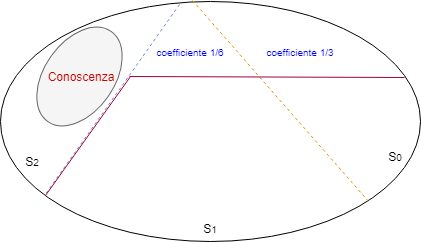
\includegraphics[width=0.60\linewidth]{./image/insieme_probabilita_rispostaesatta.png}
	\caption{Rappresentazione insiemistica della probabilit\`a di rispondere correttamente ad una domanda: P(A)}
	\label{Rappresentazione insiemistica della probabilita di rispondere correttamente ad una domanda: P(A)}
\end{figure}
  
  
  
 \paragraph{Considerazioni importanti} \mbox{}\\\\
 \label{Considerazioni importanti}
 \noindent
  In conclusione P(A)=$\frac{1}{3}+\frac{1}{6}P(S_1)+\frac{2}{3}P(S_2)$.
  Ovvero la probabilit\`a  per un candidato di dare in una domanda A la risposta corretta dipende dai seguenti fattori:
  \begin{itemize}
  \item $\frac{1}{3}$: coefficiente che rappresenta la probabilit\`a effettiva per chi non conosce la risposta alla domanda di dare la risposta corretta;
  \item $\frac{1}{2}P(S_1)$: coefficiente che rappresenta la probabilit\`a effettiva di  dare la risposta corretta quando il candidato \`e in grado di scartare una risposta sbagliata alla domanda;
   \item $\frac{2}{3}P(S_2)$: coefficiente che rappresenta la probabilit\`a effettiva di  dare la risposta corretta quando il candidato \`e in grado di scartare due risposte sbagliate alla domanda.
  \end{itemize}
  \noindent
  Dall'analisi della tipologia di eventi di coppia e dal calcolo della probabilit\`a necessaria per poter rispondere correttamente ad una domanda, si giunge alla valenza dei seguenti assiomi:
  \begin{enumerate}
  \item Le coppie di domande A e B devono essere fra loro disgiunte, altrimenti si genererebbero situazioni di invalidit\`a dei risultati;
  \item Per rispondere correttamente ad una domanda non \`e necessario che il candidato abbia piena conoscenza di tutti gli argomenti richiesti dall'esame, ma bens\`i ne risultano sufficienti $n-1$;
  \item La probabilit\`a di conoscere \`e contenuta all'interno di $S_{2}$, in quanto se un candidato conosce \`e conseguentemente in grado, da una domanda, di scartare due risposte sbagliate.
  \end{enumerate}
  
\subsubsection{Il piano}
\label{Il piano}
\noindent
La probabilit\`a P(A) che un candidato ha in gioco nel momento in cui si approccia a rispondere ad una domanda pu\`o venire rappresentata in un piano.\\\\

\noindent
Ognuno dei tre assi cartesiani rappresenta l'insieme dei casi di scarto ($S_0$, $S_1$, $S_2$). L'intersezione tra i punti del piano indica la regione accettabile contenente il range di valori assumibili da P(A). Tale punto proiettato su ognuno dei tre assi permette l'individuazione esatta dei coefficienti delle variabili $S_0$, $S_1$, $S_2$.\\\\
Ogni porzione della regione del piano viene individuata con la seguente tecnica:
\begin{enumerate}
\item Per individuare ogni retta passante per $S_0$, $S_1$ e $S_2$ \`e necessario assumere che $S_0+S_1+S_2=1$;
\item La retta passante per $S_0$ \`e rappresentabile per mezzo delle seguenti equazioni:
\begin{center}$S0=0$ e $S_1+S_2=1$\end{center}
In questo modo l'asse $S_0$ \`e fissato a 0 e estrapolando $S_1$ e $S_2$ da $S_1=-S_2+1$  assumono valori tra (0,1). 
\begin{figure}[H]
\centering
	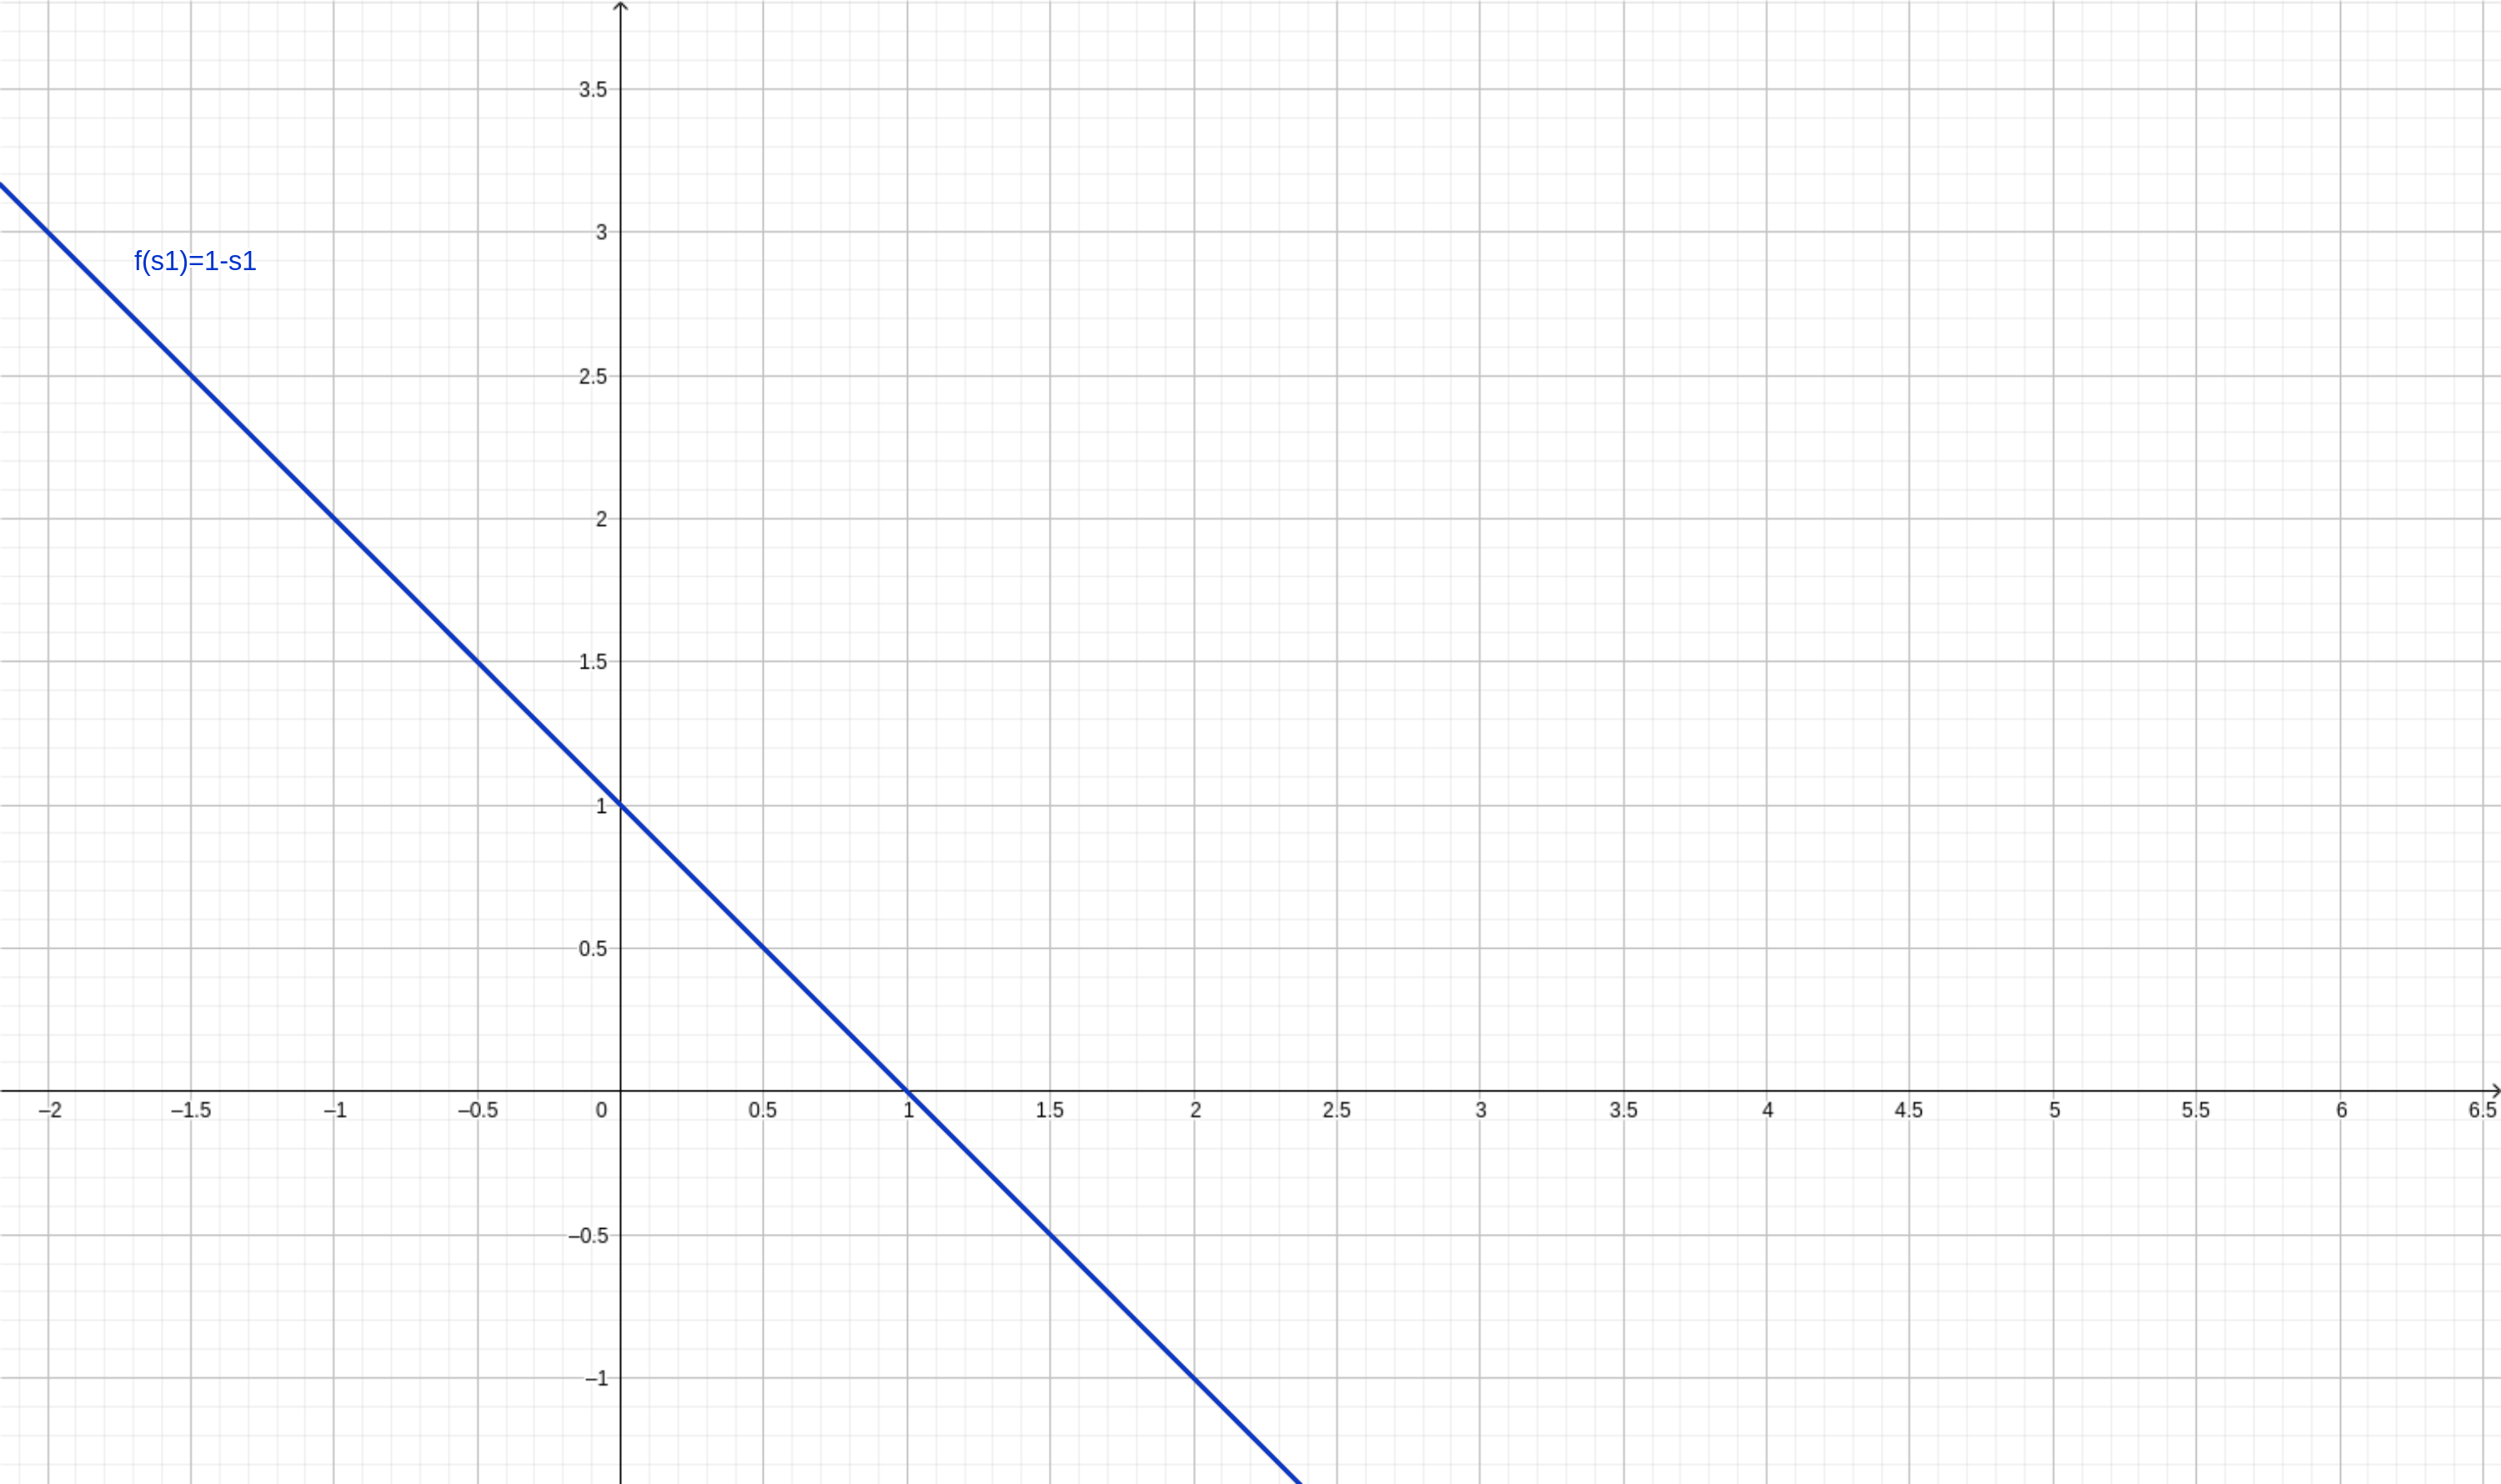
\includegraphics[width=0.90\linewidth]{./image/equazioneretta.png}
	\caption{Rappresentazione della retta passante per $S_0=0$}
	\label{Rappresentazione della retta passante per S_0=0}
\end{figure}
\item Il medesimo ragionamento vale per le rette passanti per $S_1$ e $S_2$.

\begin{center}$S_1=0$ e $S_0+S_2=1$\end{center}
l'asse $S_1$ \`e fissato a 0 e $S_0$ e $S_2$ assumono valori tra (0,1).\\\\

\begin{center} $S_2=0$ e $S_1+S_0=1$ \end{center}
l'asse $S_2$ \`e fissato a 0 e $S_0$ e $S_2$ assumono valori tra (0,1).

\item In questo modo l'unione di tutte le rette passanti per gli assi creano la regione accettabile dei valori di P(A).
\end{enumerate}

\noindent Avendo rappresentato il piano si ottiene nei punti di intersezioni fra le tre rette la regione accettabile per P(A). Inoltre \`e possibile, ora, individuare il fascio di rette che tangenti il piano permettono di affermare se una specifica domanda \`e, in base alla sua frequenza, ha difficolt\`a bassa, media, alta per un candidato.
\begin{itemize}
\item Se una domanda ha una difficolt\`a bassa la retta si situa passante per i punti $0<S_2<=1$ (molto vicino a 1) e $(S_0, S_1)<0$ (tendenti a 0);
\item Se una domanda ha una difficolt\`a alta la retta si situa passante per i punti $S_2<=0$ (molto vicino a 0), $S_1<1$ e $S_0<=1$ (tendente a non scartare alcuna risposta);
\item Se una domanda ha una difficolt\`a media la retta si situa nella parte centrale della regione accettabile, passante per i punti $0<=(S_0, S_1, S_2)<=1$.\end{itemize}

\paragraph{Rappresentazione di P(A)}\mbox\\\\

\noindent Vediamo alcuni casi di come le domande possono venire rappresentate sul piano:\\\\
La funzione di partenza \`e:
\begin{center}$F=\frac{1}{3}+\frac{1}{6}S_1+\frac{2}{3}S_2$\end{center}
Va esplicitato $S_1$, i passaggi utili da fare sono i seguenti:\\\\
$\frac{-1}{6}S_1=\frac{1}{3}+\frac{2}{3}S_2-F$ $\rightarrow$ $S_1=-4S_2-2+6F$\\\\
Essendo  che $0<=S_2<=1$ usando $S_1=1$ e $S_2=0$ si ottiene che $F=\frac{1}{2}=0.5$\\
\\
Quanto appena calcolato pu\`o venire rappresentato graficamente impiegando la retta $S_1=1-S_2$ (responsabile di definire una porzione del piano in base alle variaibili coinvolte) e mediante la retta $S_1=-4S_2-2+6F$ (che permette di calcolare il fascio di rette tangenti alla prima retta). \\

\begin{figure}[H]
\centering
	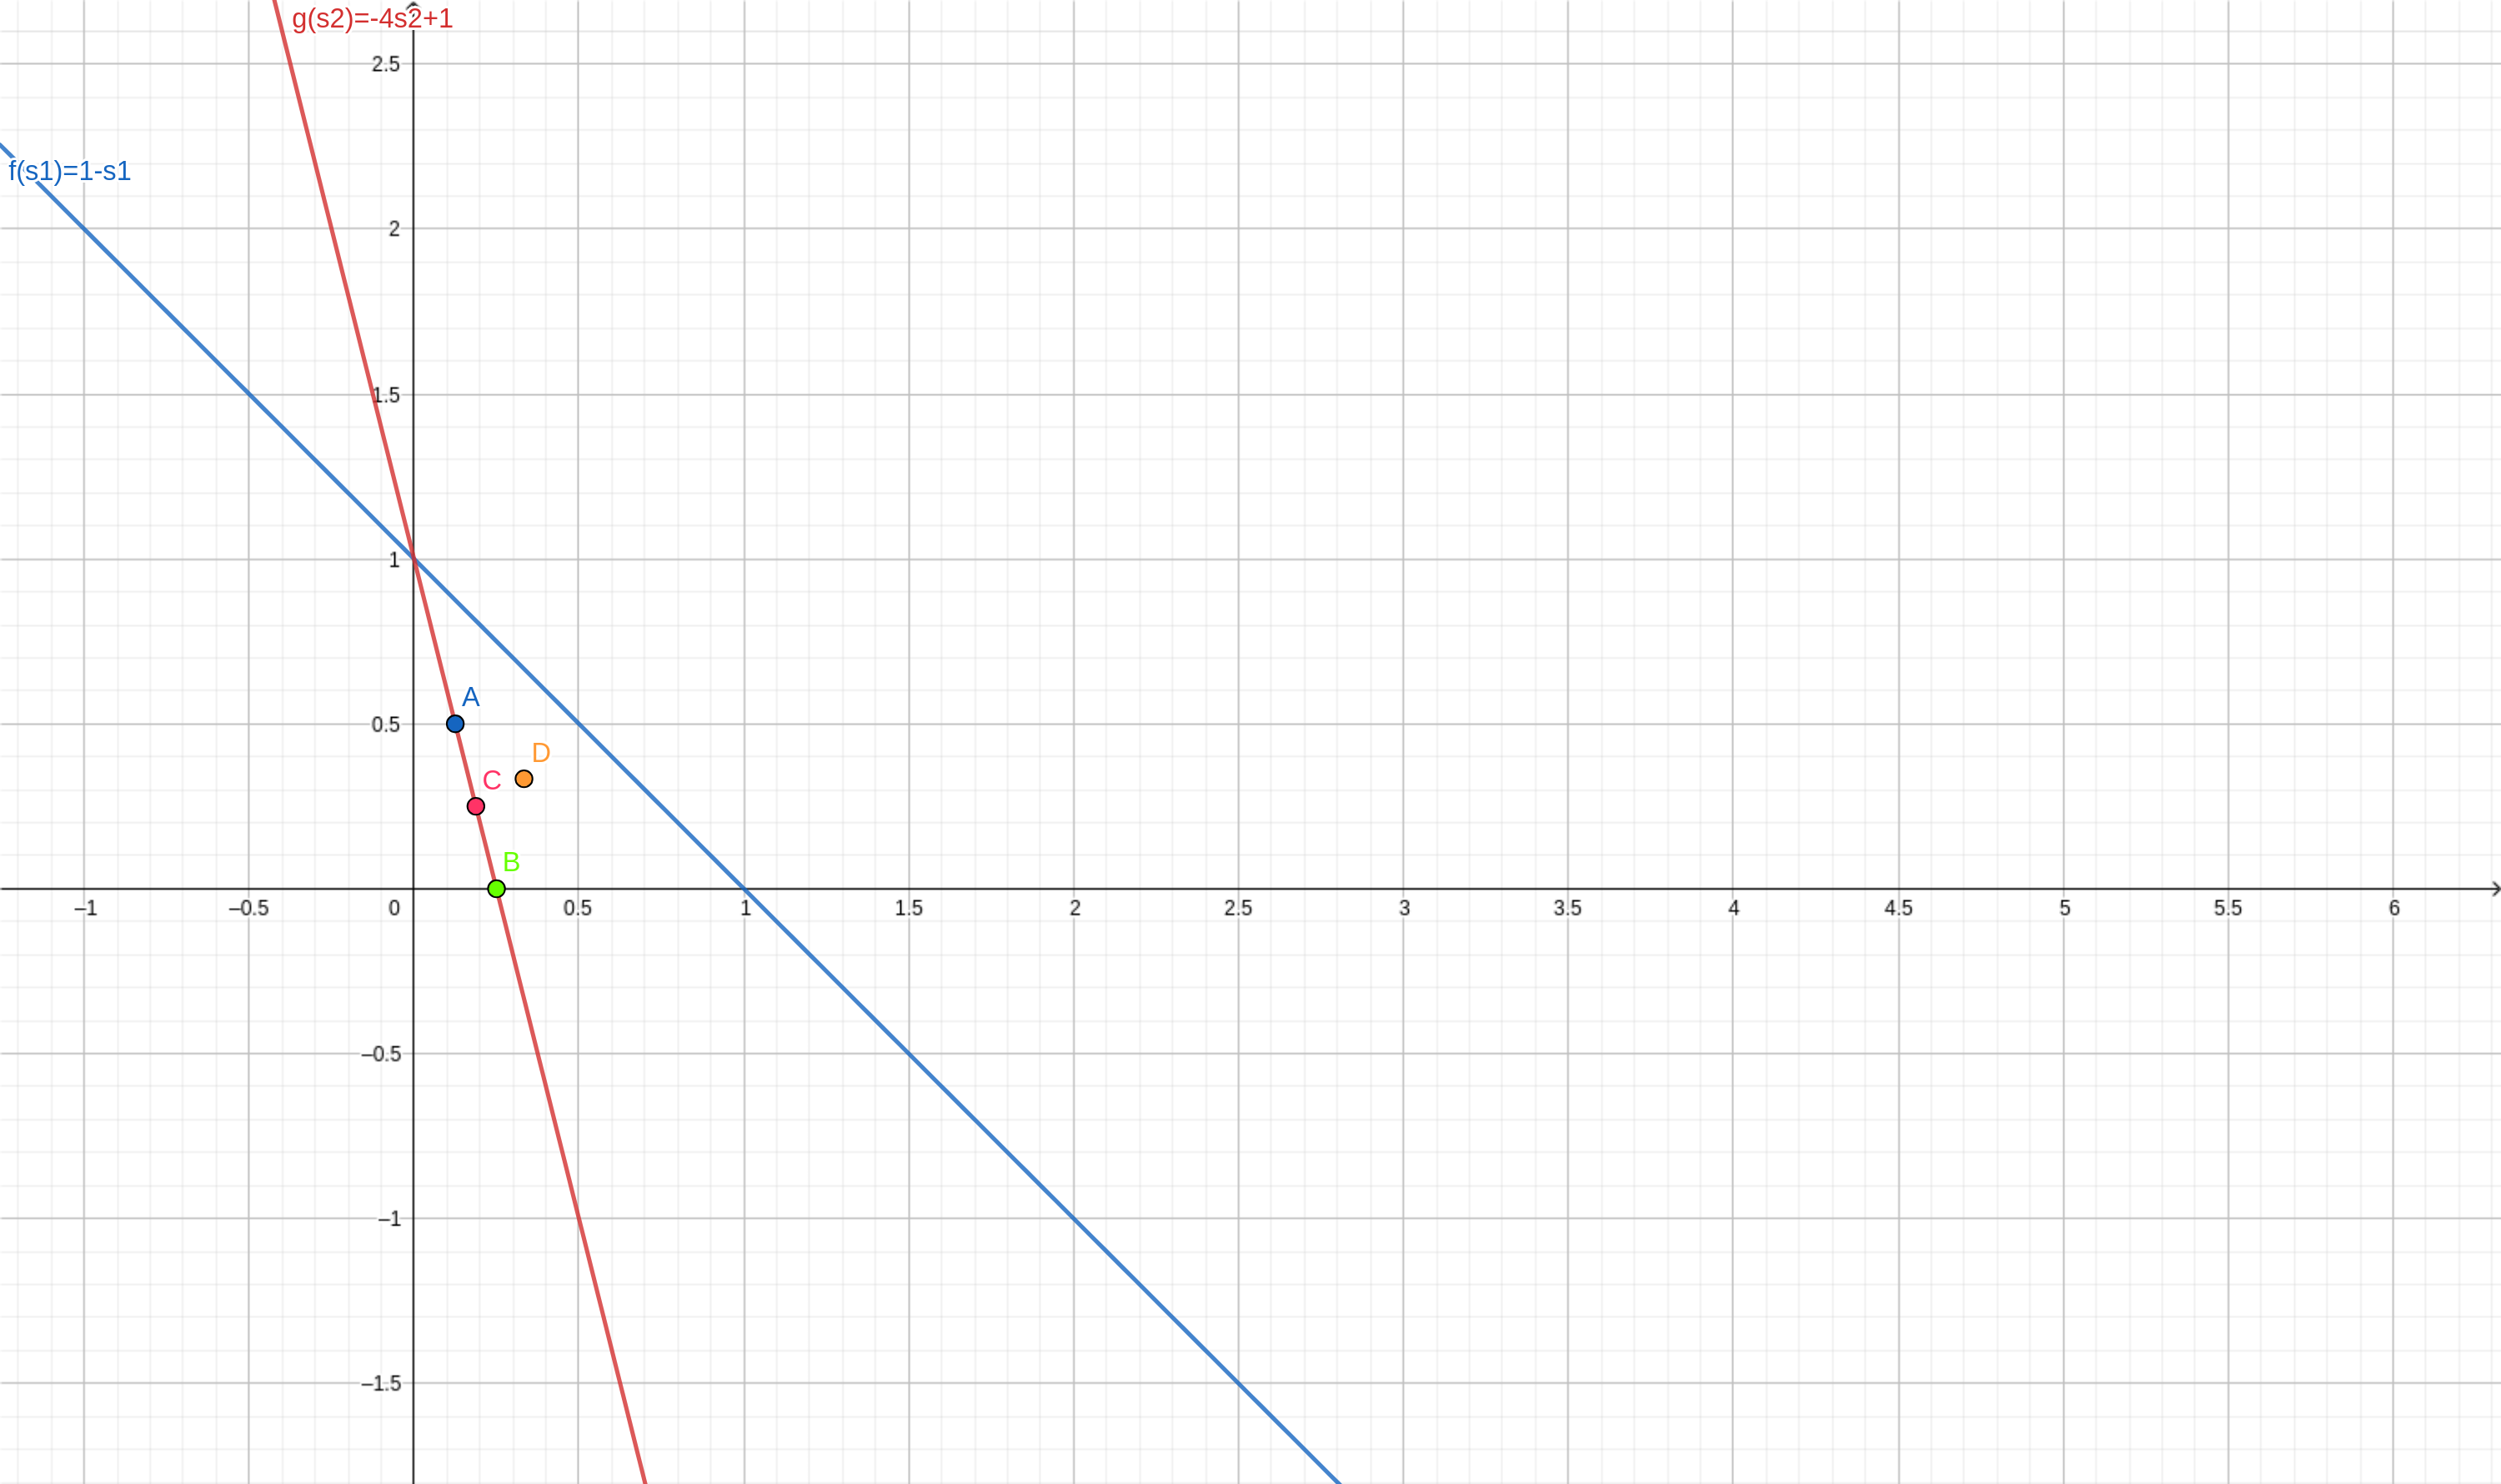
\includegraphics[width=0.90\linewidth]{./image/esempio1.png}
	\caption{Rappresentazione di P(A) per una frequenza 0.5 proiettata su assi $S_0=0$, $S_1$ e $S_2$.}
	\label{Rappresentazione di P(A) per una frequenza 0.5 proiettata su assi S_0=0, S_1 e S_2.}
\end{figure}

\noindent
Nella figura sopra sono rappresentati i seguenti significati:
\begin{itemize}
\item La linea azzurra rappresenta $S_2=1-S_1$;
\item La linea rosa rappresenta la retta tangente $S_1=-4S_2+1$;
\item Punto A (blu): \\
$S_1=0.5=\frac{1}{2}$ \\
$\frac{1}{2}=-4S_2+1$ $\rightarrow$ $4S_2=1-\frac{1}{2}$ $\rightarrow$ $S_2=\frac{1}{8}$ \\
$S_0=1-\frac{1}{2}-\frac{1}{8}=\frac{3}{8}$\\
\\
Ovvero met\`a dei candidati sottoposti alla domanda sa scartare una delle risposte, lo 0.16\% sa dare la risposta corretta e lo 0.36\% non sa scartare alcune delle risposte possibili.
\item Punto B (verde): \\
$S_1=0$\\
$S_2=\frac{1}{4}$\\
$S_0=1-\frac{1}{4}=\frac{3}{4}$\\
\\
Ovvero nessun dei candidati sottoposti alla domanda sa scartare una delle risposte, lo 0.25\% sa dare la risposta corretta e lo 0.75\% non sa scartare alcune delle risposte possibili.
\item Punto C (fucsia): \\
$S_1=\frac{1}{4}$\\
$S_2=\frac{3}{16}$\\
$S_0=1-\frac{1}{4}-\frac{3}{16}=\frac{9}{16}$\\
\\
Ovvero lo 0.25\% dei candidati sottoposti alla domanda sa scartare una delle risposte, lo 0.19\% sa dare la risposta corretta e lo 0.56\% non sa scartare alcune delle risposte possibili.
\item Punto D (arancione): \\
$S_1=\frac{1}{3}$\\
$S_2=\frac{1}{3}$\\
$S_0=1-\frac{1}{3}-\frac{1}{3}=\frac{1}{3}$\\
\\
Osserviamo che il punto in esame fuoriesce dalla regione delimitata dalla retta tangente di frequenza 0.5 ($S_1=-4S_2+1$). Conseguenza diretta data dall'impossibilit\`a di ottenere una probabilit\`a del 50\% sulla domanda con $\frac{1}{3}$ di candidati che sa scartare 2 risposte, $\frac{1}{3}$ che ne sa scartare 1 e $\frac{1}{3}$ nessuna.
\end{itemize}
\noindent
Vediamo ulteriori due esempi che permettono di valutare cosa accade nel piano nel caso di una frequenza:
\begin{enumerate} 
\item Quasi in prossimit\`a di 1;
\item Pari alla soglia minima dell'indovinato.
\end{enumerate}
\noindent

Il grafico \`e il seguente:

\begin{figure}[H]
\centering
	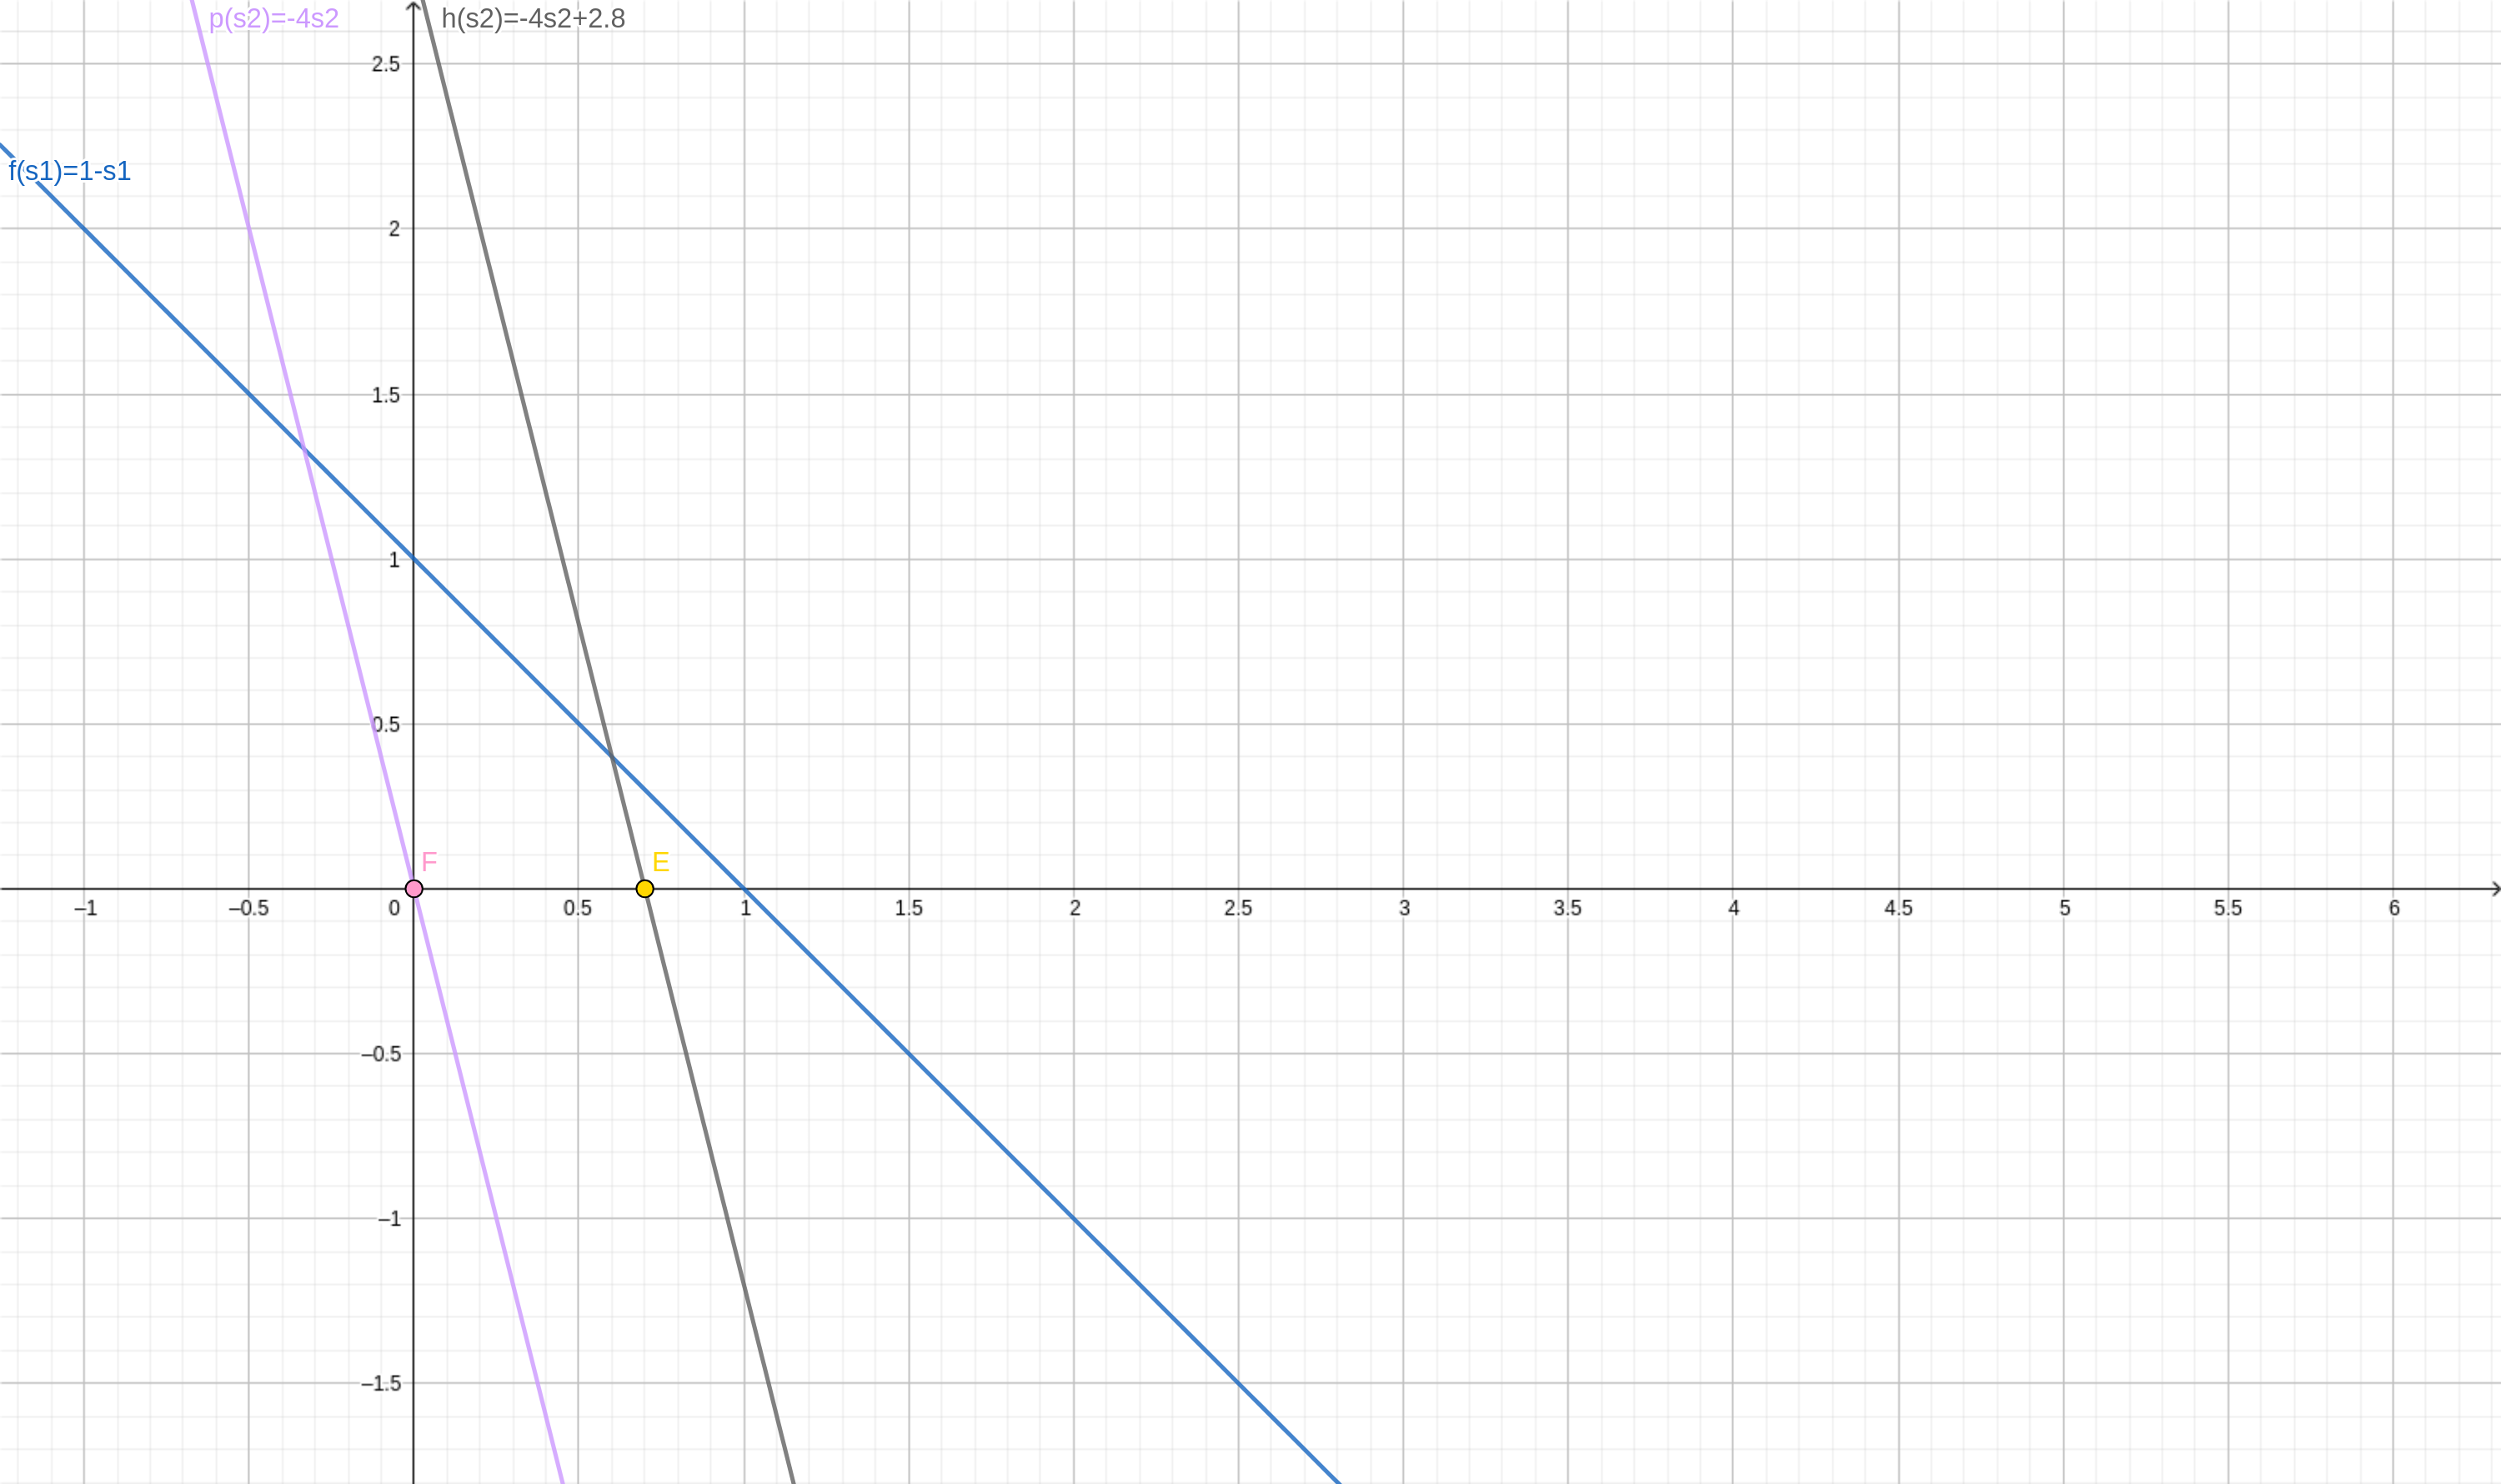
\includegraphics[width=0.90\linewidth]{./image/esempio2.png}
	\caption{Rappresentazione di P(A) per una frequenza 0.33 e 0.8 proiettate su assi $S_0=0$, $S_1$ e $S_2$.}
	\label{Rappresentazione di P(A) per una frequenza 0.33 e 0.8 proiettate su assi S_0=0, S_1 e S_2.}
\end{figure}

\begin{itemize}
\item La linea azzurra mostra la retta tangente con frequenza 0.80\%.
In questa abbiamo calcolato il punto E (giallo):\\
$S_1=0$\\
$S_2=\frac{14}{20}$\\
$S_0=0$\\
\\
Quasi la totalit\`a dei candidati ha la conoscenza per poter scartare tutte le risposte sbagliate e dare la risposta giusta alla domanda.
\item La linea viola mostra la retta tangente con frequenza 0.33\%.
In questa abbiamo calcolato il punto F (rosa):\\
$S_1=0$\\
$S_2=0$\\
$S_0=1$\\
\\ 
Ovvero nessuno dei candidati ha la conoscenza per poter scartare n\`e una n\`e due risposte, percui l'unica possibilit\`a per un candidato di rispondere alla domanda \`e indovinare. \`E evidente come se un candidato non sa la risposta ad una domanda ha una probabilit\`a dello 0.33\% di poter indovinare la risposta corretta.
\end{itemize}


\pagebreak
\section{Rete neurale}
\label{Rete neurale}

La libreria utilizzata per sviluppare la Rete neurale \`e stata \textit{ConvNetJS}. L'aspetto positivo di tale scelta \`e stata la semplicit\`a nell'utilizzo del linguaggio javascript; l'aspetto negativo ha riguardato la totale mancanza di mantenibilit\`a della libreria stessa che comporta la scarsit\`a di esempi applicativi, oltre alla documentazione ufficiale, che costringono lo sviluppatore ad una ricerca approfondita personale in un ambiente ove lo nozioni si presentano scarse e a continue prove per verificare la validit\`a del codice prodotto.
\begin{figure}[H]
\centering
	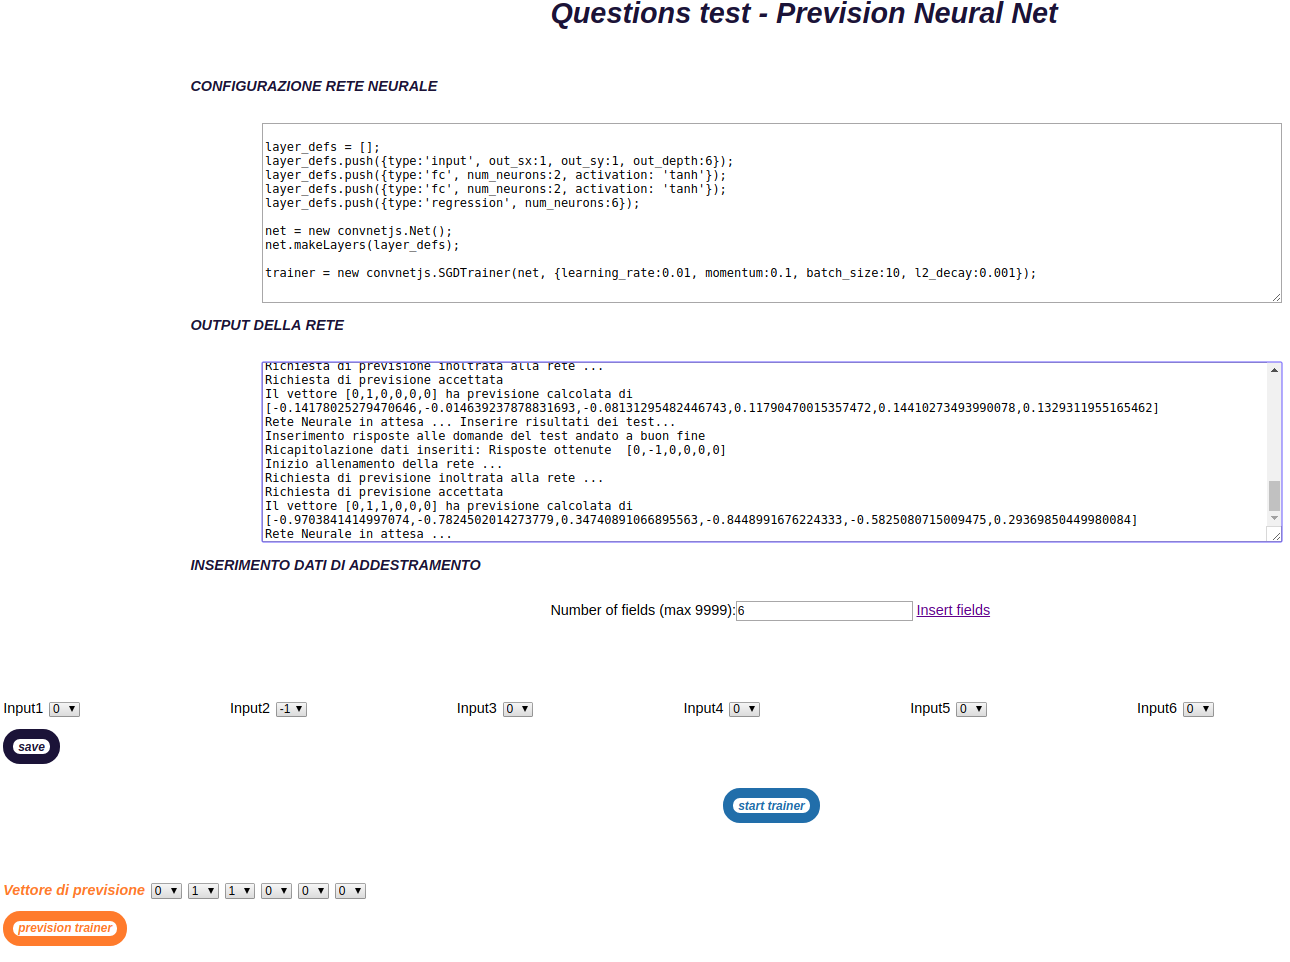
\includegraphics[width=1\linewidth]{./image/GUI-rete-neurale.png}
	\caption{Interfaccia utente della Rete neurale di prova.}
\end{figure}
\noindent
Durante il periodo 24/05 - 31/05 mi sono occupata dello sviluppo di una Rete neurale in grado di ricevere in input un training set di dimensione 6 e di restituire una previsione sui dati di apprendimento ricevuti.
\noindent
Il problema che la rete mira ad analizzare \`e quello discusso nel precedente capitolo \textit{Analisi dei dati di probabilit\`a}
\\\\
Per agevolare l'apprendimento della rete, ed ottenere delle previsioni stabili mi sono occupata di implementare due metodi di generazione randomica di dati in modo da far apprendere massicciamente la stessa.
Il dato prodotto consiste in un vettore di 6 elementi, composto da  -1, 0 e 1 con il seguente criterio:
\begin{itemize}
\item \textbf{-1}: la domanda x \`e stata posta al candidato che ha risposto in maniera errata;
\item \textbf{0}: la domanda x non \`e stata posta al candidato;
\item \textbf{1}: la domanda x \`e stata posta al candidato che ha saputo rispondere correttamente.
\end{itemize}
\noindent
Il primo metodo che ho sviluppato si occupa di generare un vettore di dati di apprendimento basandosi esclusivamente su come le domande sono interconnesse tra di loro (grazie all'uso di un grafo della conoscenza costruito ad hoc); il secondo metodo ripropone quanto perseguito dal primo metodo con il valore aggiunto di generazione di un profilo randomico di un candidato, che tiene conto della  probabilit\`a di risposta ad una domande seguendo la formula P(A)= $\frac{1}{3}+\frac{1}{6}P(S_1)+\frac{2}{3}P(S_2)$.

\subsection{Test effettuati}
\label{Test effettuati}

Alcune decisioni che ho preso durante la scelta dell'architettura della rete riguardano i seguenti settori:
\begin{enumerate}
\item Una rete neurale non deve, per fornire dei dati attendibili, possedere un numero di neuroni troppo elevato rispetto al trainset effettuato; altrimenti la previsione  ritornerebbe l'identit\`a del vettore di input della stessa, come conseguenza diretta della capacit\`a troppo elevata di immagazzinare dati.
\item I layers, ho deciso, di allenarli mediante tecnica di regressione, che permette l'inserimento in input di una funzione obiettivo e l'ottenimento di un risultato, in output, anche in virgola mobile e composto di tanti elementi quanti sono i neuroni di regressione dichiarati. Per la mia rete di prova \`e necessario dichiarare  6 neuroni in regressione perch\`e l'output, appunto, che ci si aspetta dal sistema \`e di 6 elementi.
\item Per costruire un dataset di dati consistente che permettesse alla rete di imparare qualcosa ho costruito un grafo della conoscenza con lo scopo di mettere in relazione degli argomenti che coinvolgono uno o pi\`u domande.
\begin{figure}[H]
\centering
	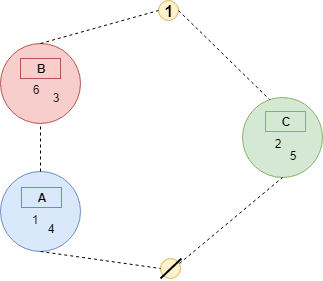
\includegraphics[width=0.60\linewidth]{./image/grafo_trainset.png}
	\caption{Grafo rappresentante le relazioni esistenti tra il set di domande di prova.}
\end{figure}
\noindent
Per svolgere l'apprendimento ogni vettore, facente parte del dataset, viene dato in pasto alla rete che a sua volta provvede alla sua assimilazione come conoscenza mediante la tecnica dell'autoencoder, ovvero la rete impara il vettore riducendone lo spazio occupato.
\item Per creare il dataset ho ritenuto sufficiente generare \textit{2000} vettori di risposta in modo da compiere in maniera esaustivo l'apprendimento della rete.
\end{enumerate}
\noindent
Il vettore passato in input per svolgere le previsioni \`e \textit{[0,0,0,0,0,0]},\textit{[0,0,1,0,1,0]} e \textit{[0,0,-1,0,0,0]}\\
Le aspettative riguardano la previsione di risposta di un candidato
\noindent. 
Di seguito riporto quanto \`e stato rilevato in fase di test.

\subsubsection{Architettura  della rete: 4 neuroni per ciascuno dei 2 layers}
\label{Configurazione della rete: 4 neuroni per ciascuno dei 2 layers}

Architettura  della rete utilizzata:\\
\begin{verbatim}layer_defs = [];
layer_defs.push({type:'input', out_sx:1, out_sy:1, out_depth:6});
layer_defs.push({type:'fc', num_neurons:4, activation: 'tanh'});
layer_defs.push({type:'fc', num_neurons:4, activation: 'tanh'});
layer_defs.push({type:'regression', num_neurons:6});

net = new convnetjs.Net();
net.makeLayers(layer_defs);

trainer = new convnetjs.SGDTrainer(net, {learning_rate:0.01,
 momentum:0.1, batch_size:10, l2_decay:0.001});
\end{verbatim}
\noindent
I layers utilizzati sono 2 e compositi da 4 neuroni.

\paragraph{Training set standard a 4 neuroni per ciascuno dei 2 layers}\mbox{}
\label{Training set standard a 4 neuroni per ciascuno dei 2 layers}
\\
\noindent
\begin{itemize}
\item \begin{verbatim}Il vettore [0,0,0,0,0,0] ha previsione calcolata di
[-0.021598804903572744,-0.1372509042342871,0.06611969158456255,
0.018121335417653706,-0.11264571886853292,0.17520370837747462]\end{verbatim}
Appaiono in relazione le domande 1, 2, 5 e 3, 4, 6.\\
Gli scostamenti tra le coppie 2, 5 e 3, 6 sono consistenti con quelle che sono le relazioni di dipendenza, invece 1, 4 ha una differenza di 0.016 circa che parte da qualche millesimo fino 0.5
Le domande 3 e 6 si dovrebbero presentare con una positivit\`a inferiore rispetto a 1 e 4; nel test in analisi questo non viene rispettato da nessuna delle coppie in analisi per differenze che vanno da qualche millesimo fino a 0.018 circa.
\paragraph{Osservazioni}\mbox{}
\label{Osservazioni su rete a 4 neuroni per ciascuno dei 2 layers}
\\\\
\noindent
L'architettura testata si compone di 4 neuroni a layer su una base di 2000 test correndo il rischio di avere una rete che apprende troppo e come effetto negativo "veda" addirittura cose che non esistono. A prova di ci\`o sono i risultati non conformi alle attese.
Dunque mi fermo qui con il test di tale architettura e riducendone il numero di neuroni presenti in ciascun layers e/o il numero di layers presenti.\\

Le nuove architetture su cui ho effettuato i test sono esposte nei paragrafi seguenti.

\subsubsection{Architettura della rete a 2 neuroni per ciascuno dei 2 layers}
\label{Architettura della rete a 2 neuroni per ciascuno dei 2 layers}
Architettura  della rete utilizzata:\\
\begin{verbatim}layer_defs = [];
layer_defs.push({type:'input', out_sx:1, out_sy:1, out_depth:6});
layer_defs.push({type:'fc', num_neurons:2, activation: 'tanh'});
layer_defs.push({type:'fc', num_neurons:2, activation: 'tanh'});
layer_defs.push({type:'regression', num_neurons:6});

net = new convnetjs.Net();
net.makeLayers(layer_defs);

trainer = new convnetjs.SGDTrainer(net, {learning_rate:0.01,
 momentum:0.1, batch_size:10, l2_decay:0.001});
\end{verbatim}
\noindent
I layers utilizzati sono 2 compositi da 2 neuroni.

\paragraph{Training set standard su rete a 2 neuroni per ciascuno dei 2 layers}\mbox{}
\label{Training set standard su rete a 2 neuroni per ciascuno dei 2 layers}
\\
\noindent
\begin{itemize}
\item \begin{verbatim}[Il vettore [0,0,0,0,0,0] ha previsione calcolata di
[0.31232372051574936,0.7253754889487585,-0.5051208979797573,
0.32075742158673093,0.7324947496336937,-0.4348299972940168]
\end{verbatim}
Appaiono in relazione le domande 1, 2, 4, 5 e 3, 6.\\
Gli scostamenti tra le coppie 1, 4 e 3, 6  e 2, 5 sono consistenti con quelle che sono le relazioni di dipendenza fra le domande.
Le domande 3 e 6 si dovrebbero presentare con una positivit\`a inferiore rispetto a 1 e 4; in questo test la regola viene rispettata pienamente.\\
Dai dati della previsione si nota come il candidato ha una buona probabilit\`a di saper rispondere alla coppia 1 e 4, e ancora pi\`u elevata di saper rispondere correttamente alla coppia 2 e 5; molto bassa di saper rispondere correttamente alle 3 e 6 che sono, appunto, di una difficolt\`a maggiore rispetto alla coppia 1 e 4.

\item \begin{verbatim}Il vettore [0,0,1,0,1,0] ha previsione calcolata di
[0.5123144717131076,0.9123354449531641,0.2837937822420923,
0.46449868699771607,0.9029832167165894,0.3227303792035435]
\end{verbatim}
Appaiono in relazione le domande 1, 2, 3  4, 5, 6.\\
Gli scostamenti tra le coppie 1, 4 e 3, 6  e 2, 5 sono consistenti con quelle che sono le relazioni di dipendenza fra le domande.
Le domande 3 e 6 si dovrebbero presentare con una positivit\`a inferiore rispetto a 1 e 4; in questo test la regola viene rispettata pienamente.\\
Dai dati della previsione si nota come il candidato ha un'ottima probabilit\`a di saper rispondere alla coppia 2 e 5 (come imposto dal vettore previsione), buona di saper rispondere alla coppie 3 e 6 (come imposto dal vettore previsione) e pi\`u che buona  di saper rispondere alle 1 e 4, che sono di una semplicit\`a pi\`u elevata rispetto alla 3 e 4.
\end{itemize}

\item \begin{verbatim}Il vettore [0,0,-1,0,0,0] ha previsione calcolata di
[0.3698539826215957,0.288907514487717,-0.8504159455662308,
0.3663192502433841,0.2937448801761998,-0.7845589473185985]
\end{verbatim}
Appaiono in relazione le domande 1, 2, 4, 5 e 3, 6.\\
Gli scostamenti tra le coppie 1, 4 e 3, 6  e 2, 5 sono consistenti con quelle che sono le relazioni di dipendenza fra le domande.
Le domande 3 e 6 si dovrebbero presentare con una positivit\`a inferiore rispetto a 1 e 4; in questo test la regola viene rispettata pienamente.\\
Dai dati della previsione si nota come il candidato ha una discreta probabilit\`a di saper rispondere alla coppia 2 e 5, un p\`o meglio di saper rispondere alla coppie 1 e 4 e pi\`u di non saper saper rispondere alle 3 e 6 (come imposto dal vettore previsione).
\end{itemize}

\paragraph{Training set con generazione del profilo di un candidato e calcolo delle probabilit\`a di risposta a 2 neuroni per ciascuno dei 2 layers}\mbox{}
\label{Training set con generazione del profilo di un candidato e calcolo delle probabilita di risposta a 2 neuroni per ciascuno dei 2 layers}
\\
\noindent
\begin{itemize}
\item \begin{verbatim}Il vettore [0,0,0,0,0,0] ha previsione calcolata di
[0.057781303506280995,0.0513731100126314,-0.06600467867066256,
0.029940883111932555,-0.019564515397168573,-0.09570617900597932]
\end{verbatim}
Appaiono in relazione le domande 1, 2, 4 e 3, 5, 6.\\
Gli scostamenti tra la coppia 1, 4 e 3, 6 sono consistenti con  quelle che sono le relazioni di dipendenza fra le domande; invece per la coppia 2 e 5 i segni sono opposti con una differenza di 0.024.
Le domande 3 e 6 si dovrebbero presentare con una positivit\`a inferiore rispetto a 1 e 4, la regola viene rispettata pienamente. Le anomalie riscontrate sono da ricondurre alla natura del vettore di training che si basa sul calcolo della probabilit\`a di una risposta che sul grafo della conoscenza.

\item \begin{verbatim}Il vettore [0,0,1,0,1,0] ha previsione calcolata di
[0.19494624113789977,0.1712744021266377,0.577963304906936,
0.781098215373483,0.3774535909060714,0.03617314870307162]
\end{verbatim}
Appaiono in relazione le domande 1, 2, 3, 4, 5, 6.\\
Gli scostamenti tra le coppie 1 e 4 , 2 e 5, 3 e 6 sono consistenti con quelle che sono le relazioni di dipendenza fra le domande.
Le domande 3 e 6 si dovrebbero presentare con una positivit\`a inferiore rispetto a 1 e 4, la regola non viene rispettata dalla domanda 1 in rapporto con la domanda per una differenza di 0.37 circa.
Le anomalie riscontrate sono da ricondurre alla natura del vettore di training che si basa sul calcolo della probabilit\`a di una risposta che sul grafo della conoscenza.

\item \begin{verbatim}Il vettore [0,0,-1,0,0,0] ha previsione calcolata di
[0.09845785763965222,0.015421380649956663,-0.5138068038427066,
-0.4853190165287735,-0.22629262719814794,0.0008152164571250502]
\end{verbatim}
Appaiono in relazione le domande 1, 2, 6 e 3, 4, 5.\\
Gli scostamenti tra le coppie 1, 4 e 2, 5 e 3, 6 per una differenza tuttavia trascurabile  che oscilla dallo 0.2 allo 0.5.
Le domande 3 e 6 si dovrebbero presentare con una positivit\`a inferiore rispetto a 1 e 4, la regola non vale per la coppa 6 e 4.
Le anomalie riscontrate sono da ricondurre alla natura del vettore di training che si basa sul calcolo della probabilit\`a di una risposta che sul grafo della conoscenza.
\end{itemize}


\paragraph{Osservazioni}\mbox{}
\label{Osservazioni su rete a 2 neuroni per ciascuno dei 2 layers}
\\\\
\noindent
Confrontando i risultati ottenuti dalla rete con i layers impostati a 4 neuroni con quanto emerso dai dati risultanti dalla  rete a 2 neuroni emerge come l'architettura  a 2 neuroni a layers \`e sicuramente quella che da i risultati attesi.\\
Quanto emerso di discordate dal secondo training set \`e come da aspettative da associare alla natura stessa della creazione del set di dati.


\subsubsection{Architettura della rete a 4 neuroni per 1 layer}
\label{Architettura della rete a 4 neuroni per 1 layer}

Architettura della rete utilizzata:\\
\begin{verbatim}layer_defs = [];
layer_defs.push({type:'input', out_sx:1, out_sy:1, out_depth:6});
layer_defs.push({type:'fc', num_neurons:4, activation: 'tanh'});
layer_defs.push({type:'regression', num_neurons:6});

net = new convnetjs.Net();
net.makeLayers(layer_defs);

trainer = new convnetjs.SGDTrainer(net, {learning_rate:0.01,
 momentum:0.1, batch_size:10, l2_decay:0.001});
\end{verbatim}
\noindent
Viene utilizzato un unico layer da 4 neuroni.

\paragraph{Training set standard su rete a 4 neuroni per 1 layer}\mbox{}
\label{Training set standard su rete a 4 neuroni per 1 layer}
\\
\noindent
\begin{itemize}
\item \begin{verbatim}Il vettore [0,0,0,0,0,0] ha previsione calcolata di
[0.12202628618565468,0.08221724740100582,0.02233631914718809,
0.09586625658118901,0.05558075220027264,0.13443779128784109]
\end{verbatim}
Appaiono in relazione le domande 1, 2, 3, 4, 5, 6.\\
Gli scostamenti tra le coppie 1, 4 e 3, 6  e 2, 5 sono consistenti con quelle che sono le relazioni di dipendenza fra le domande.
Le domande 3 e 6 si dovrebbero presentare con una positivit\`a inferiore rispetto a 1 e 4; in questo test la regola non viene rispettata dalla domanda 6.\\
Dai dati della previsione si nota come il candidato non ha una buona probabilit\`a di saper rispondere alle domande  e la domanda 6 non si presenta conforme alle aspettative.
\end{itemize}

\paragraph{Osservazioni}\mbox{}
\label{Osservazioni su rete a 4 neuroni per 1 layer}
\\\\
\noindent
\textit{Rispetto a quanto osservato nei casi precedenti, ancora l'architettura  che rispetta le attese \`e quella con 2 neuroni per 2 layers.}
\\\\
\noindent
Tale conclusione ha perfettamente senso in quanto il grafo della conoscenza che ho usato come base per costruire i vettori di apprendimento \`e composto da 3 nodi (A, B, C) indicanti 3 neuroni; il quarto pu\`o venire valutato come un nodo della rete utile per parametri in entrata e in uscita.
\\\\
Per estendere maggiormente la mia conoscenza della rete, ho provveduto ad aumentare progressivamente il numero di neuroni a layers e osservarne le interazioni. Svolgendo ci\`o mi sono accorta che il risultato ottenuto dalla previsione era il pi\`u possibile vicino al vettore previsione; conseguenza diretta di un numero eccessivo di neuroni dati alla rete per l'apprendimento rispetto al training set svolto, generatrice di una situazione di overfitting e non attendibilit\`a dei dati raccolti.
L'architettura a 1 e 2 neuroni invece presenta una buona capacit\`a di previsione in quasi tutti i casi, per\`o tende ad andare in overfitting, come riporto di seguito:
\begin{verbatim}
Il vettore [0,0,0,0,0,1] ha previsione calcolata di
[0.5613347853884025,0.8310670629630683,-1.03049430206139,
0.5492731069379962,0.5679700877862532,-0.8637707232817535]
\end{verbatim}
Il numero di neuroni non \`e sufficiente per memorizzare che la domanda 6 deve essere positiva, e comporta a cascata la correttezza anche delle domande 3, 4 e 1. La situazione si presenta simile se il layer con 1 neurone \`e posto al di sotto.


\subsection{Sviluppo della rete delle domande nel database aziendale}
\label{Sviluppo della rete del database}

\subsubsection{Montaggio e configurazione della rete}
\label{Montaggio e configurazione della rete}

Durante la settimana dal 03/06 al 07/06 la mia attivit\`a principale \`e stata il montaggio e la configurazione della Rete neurale inerente il database aziendale con dataset i colloqui ai candidati.
Inoltre ho rivolto parte delle ore a modificare e ottimizzare quanto gi\`a implementato nella Rete di prova, in modo che ogni cosa implementata sulla rete del database \`e presenta anche in versione ridotta.\\\\
Per rendere pi\`u comprensibile le previsioni di probabilit\`a ottenute, a seguito dell'addestramento della rete e della data in pasto del vettore previsione, ho realizzato un'immagine canvas in cui ogni domanda viene raffigurata con un quadrattino colorato in base alla previsione risultante (verde se a 1, bianco a 0, rosso a -1, gradazioni di bianco - verde e bianco - rosso per i valori intermedi.
\begin{figure}[H]
\centering
	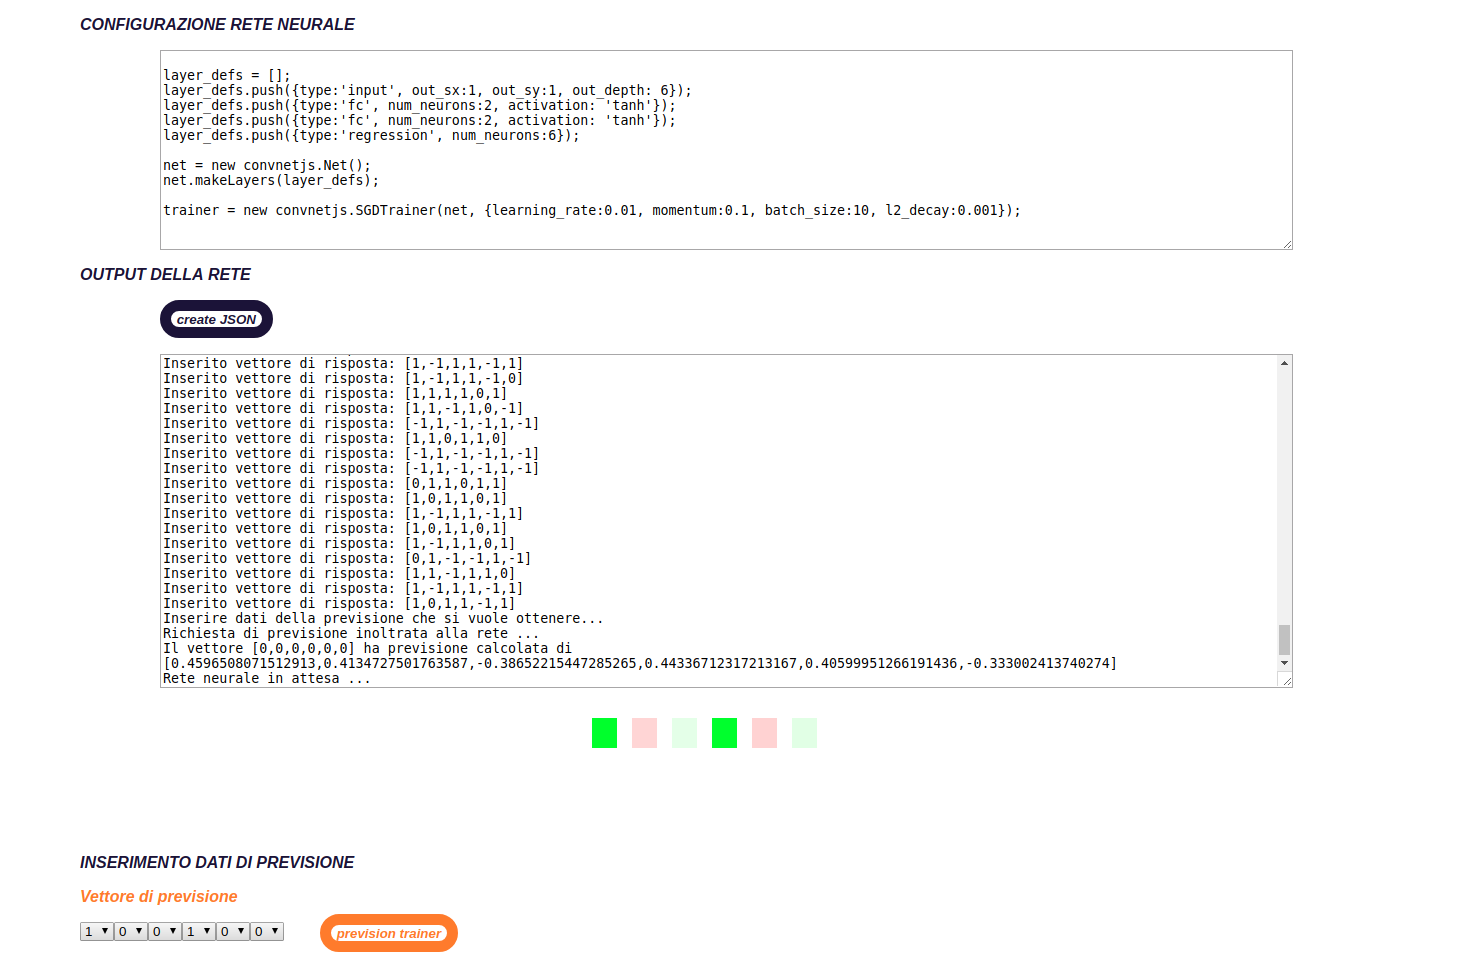
\includegraphics[width=0.90\linewidth]{./image/rete_prova-canvas.png}
	\caption{Rete di prova dopo lo sviluppo del canvas per le previsioni.}
\end{figure}

\begin{figure}[H]
\centering
	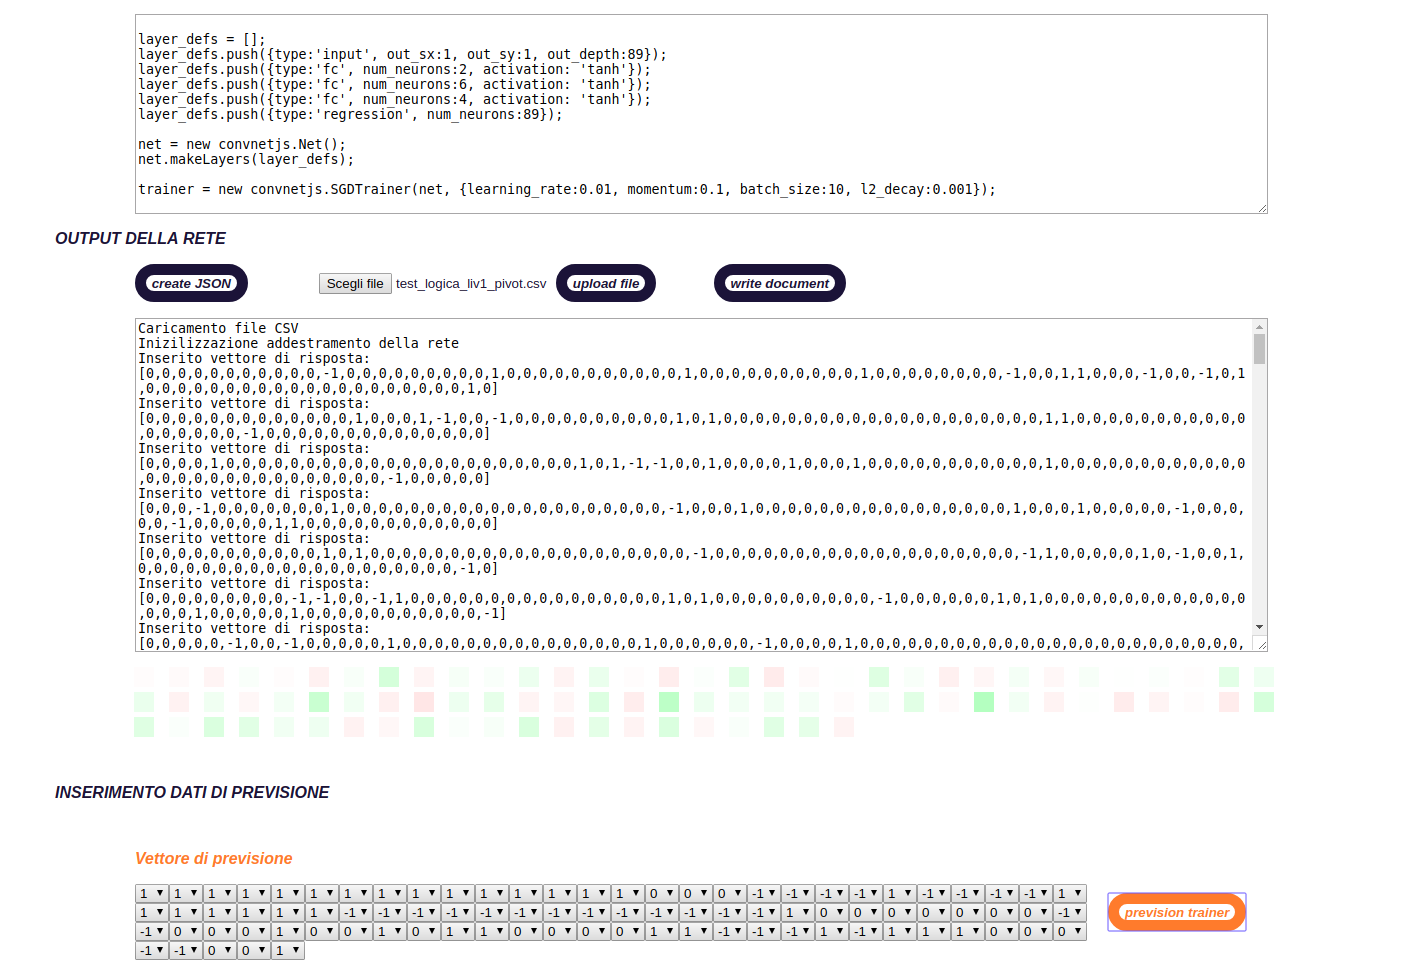
\includegraphics[width=0.90\linewidth]{./image/rete_db.png}
	\caption{Rete neurale del database aziendale.}
\end{figure}
\noindent
L'architettura che ho utilizzato, basandomi anche sul quanto appreso dalla rete neurale di prova e dal numero di vettori di test utilizzati (1245 vettori x 89) ho aumentato le dimensioni della rete.
\begin{verbatim}
layer_defs = [];
layer_defs.push({type:'input', out_sx:1, out_sy:1, out_depth:89});
layer_defs.push({type:'fc', num_neurons:2, activation: 'tanh'});
layer_defs.push({type:'fc', num_neurons:6, activation: 'tanh'});
layer_defs.push({type:'fc', num_neurons:4, activation: 'tanh'});
layer_defs.push({type:'regression', num_neurons:89});

net = new convnetjs.Net();
net.makeLayers(layer_defs);

trainer = new convnetjs.SGDTrainer(net, {learning_rate:0.01,
momentum:0.1, batch_size:10, l2_decay:0.001});
\end{verbatim}
Ho aggiunto un layer e messo un numero di neuroni per layer in modo da formare un romboide. Devo verificare la bont\`a di questa mia scelta o se invece mi porta ad una situazione di overfitting.

\noindent
Analizzando il training set dei vettori ho riscontrato tali correlazioni:
\begin{itemize}
\item Solo una piccola parte delle domande presenti in un database vengono svolte durante un colloquio con un candidato, in media una decina su 89 possibili;
\item Dalla rete sembra che le domande abbiano qualche correlazione, tuttavia la configurazione attuale ne rende difficoltosa l'individuazione.
\end{itemize}


\subsubsection{Test e Documentazione}
\label{Test e Documentazione}
Durante la settimana dal 10/06 al 18/06 ho effettuato quanto definito al interno del Piano di Lavoro come "Test e Documentazione".

\paragraph{Test nella Rete di prova}\mbox{}\\\\
\label{Test nella Rete di prova}
\noindent
Architettura della rete utilizzata:\\
\begin{verbatim}layer_defs = [];
layer_defs.push({type:'input', out_sx:1, out_sy:1, out_depth:6});
layer_defs.push({type:'fc', num_neurons:2, activation: 'tanh'});
layer_defs.push({type:'fc', num_neurons:2, activation: 'tanh'});
layer_defs.push({type:'regression', num_neurons:6});

net = new convnetjs.Net();
net.makeLayers(layer_defs);

trainer = new convnetjs.SGDTrainer(net, {learning_rate:0.01,
 momentum:0.1, batch_size:10, l2_decay:0.001});
\end{verbatim}
\noindent



\begin{itemize}
\item \begin{verbatim}Il vettore [1,1,1,1,1,1] ha previsione calcolata di
[0.8521066399598267,0.898137375081856,0.9993098151218291,0.792190337086403,
0.811145866789799,0.9514731560722426]
\end{verbatim}

\begin{figure}[H]
\centering
	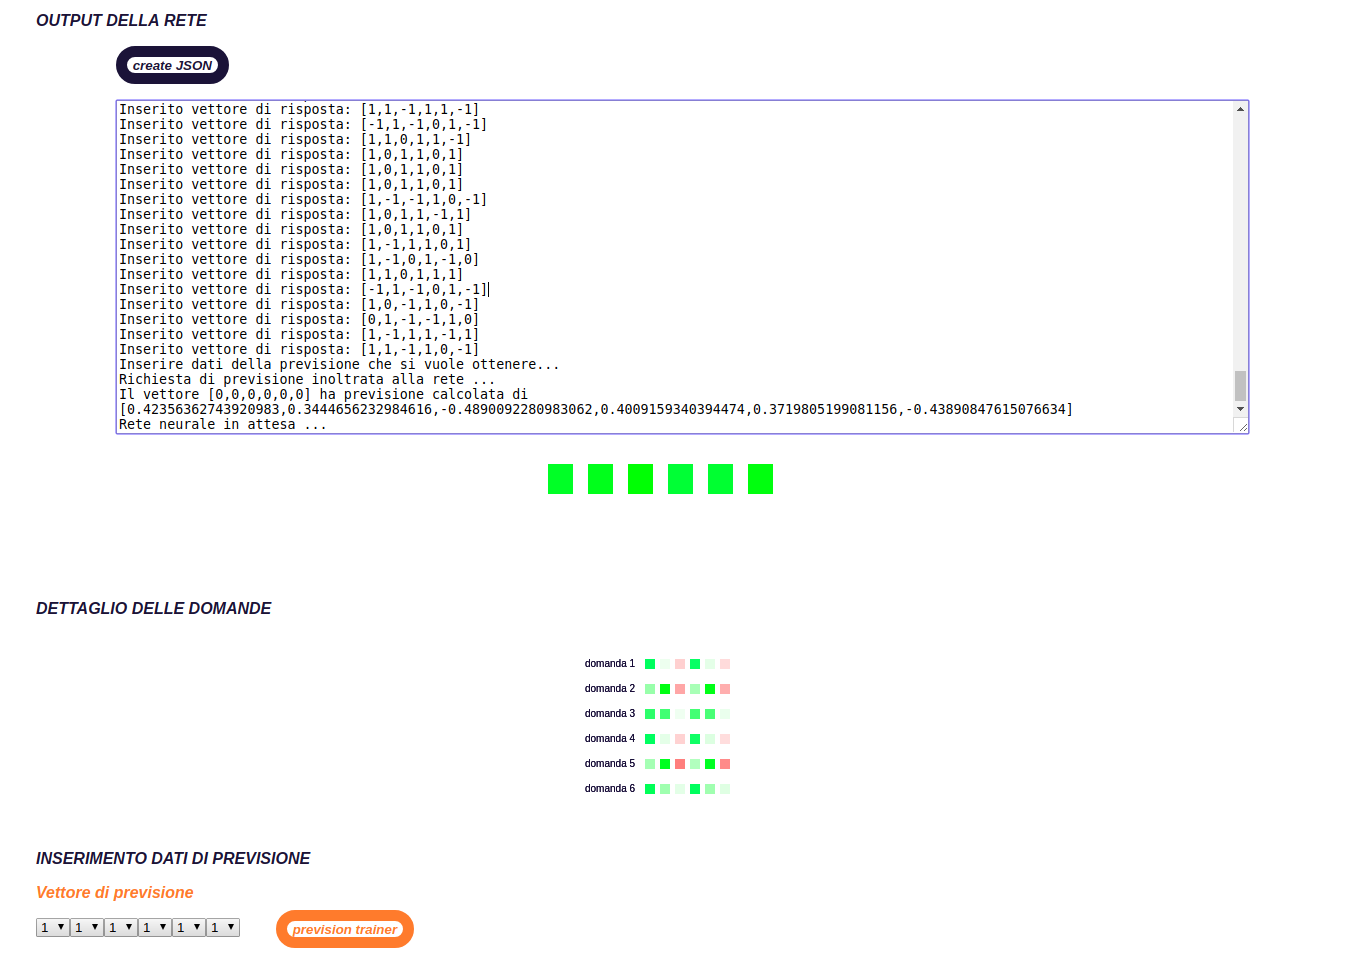
\includegraphics[width=0.90\linewidth]{./image/rete_prova-vp1.png}
	\caption{Risultato della rete di prova a seguito di un vettore di previsione [1, 1, 1, 1, 1, 1] in input.}
\end{figure}
Quanto mostrato dal dettaglio delle domande ha il seguente significato per un candidato:
\begin{itemize}
\item \textit{se la domanda 1 \`e settata a 1 (corretta)}: la rete prevede che la domanda 1 e 4 abbiano una probabilit\`a alta di essere risposte in modo corretto (verde); la 3 e 6 una probabilit\`a non eccessiva di venire risposte in modo sbagliato (rosa attenuato), la 2 e la 5 di non venire nemmeno poste (bianco con qualche minima sfumatura di verde).
\item \textit{se la domanda 2 \`e settata a 1 (corretta)}: la rete prevede che la domanda 1 e 4 abbiano una probabilit\`a non molto alta di essere risposte in modo corretto (bianco con qualche sfumatura di verde); la 3 e 6 una buona probabilit\`a di venire risposte in modo sbagliato (rosa), la 2 e la 5 di venire date in modo corretto (verde).
\item \textit{se la domanda 3 \`e settata a 1 (corretta)}: la rete prevede che la domanda 3 e 6 abbiano una probabilit\`a comunque bassa di essere risposte in modo corretto (bianco con qualche sfumatura di verde); la 1 e 4 con probabilit\`a di venire risposte in modo corretto (verde) perch\`e pi\`u semplici delle domande 3 e 6, la 2 e la 5 di venire risposte correttamente (verde).
\item \textit{se la domanda 4 \`e settata a 1 (corretta)}: la rete prevede un risultato  identico a quanto ottenuto dalla domanda 1.
\item \textit{se la domanda 5 \`e settata a 1 (corretta)}: la rete prevede un risultato similare a quanto ottenuto dalla domanda 2. Cambia solo quanto previsto dalle domande 3 e 6 che si presentano con un rosa un p\`o pi\`u intenso, in quanto con correlate alla coppia di domande 2 e 5.
\item \textit{se la domanda 6 \`e settata a 1 (corretta)}: la rete prevede un risultato simile a quanto ottenuto dalla domanda 3. La coppia 2 e 5 hanno una probabilit\`a minore di essere date correttamente (bianco con sfumature di verde) ma perch\`e non correlate alle domande 3 e 6.
\end{itemize}

\item \begin{verbatim}Il vettore [-1,-1,-1,-1,-1,-1] ha previsione calcolata di
[0.3440856175367477,-0.5026946644729329,-1.284368009920025,
0.35883842020377565,-0.37844446052773495,-1.1717763012412878]
\end{verbatim}

\begin{figure}[H]
\centering
	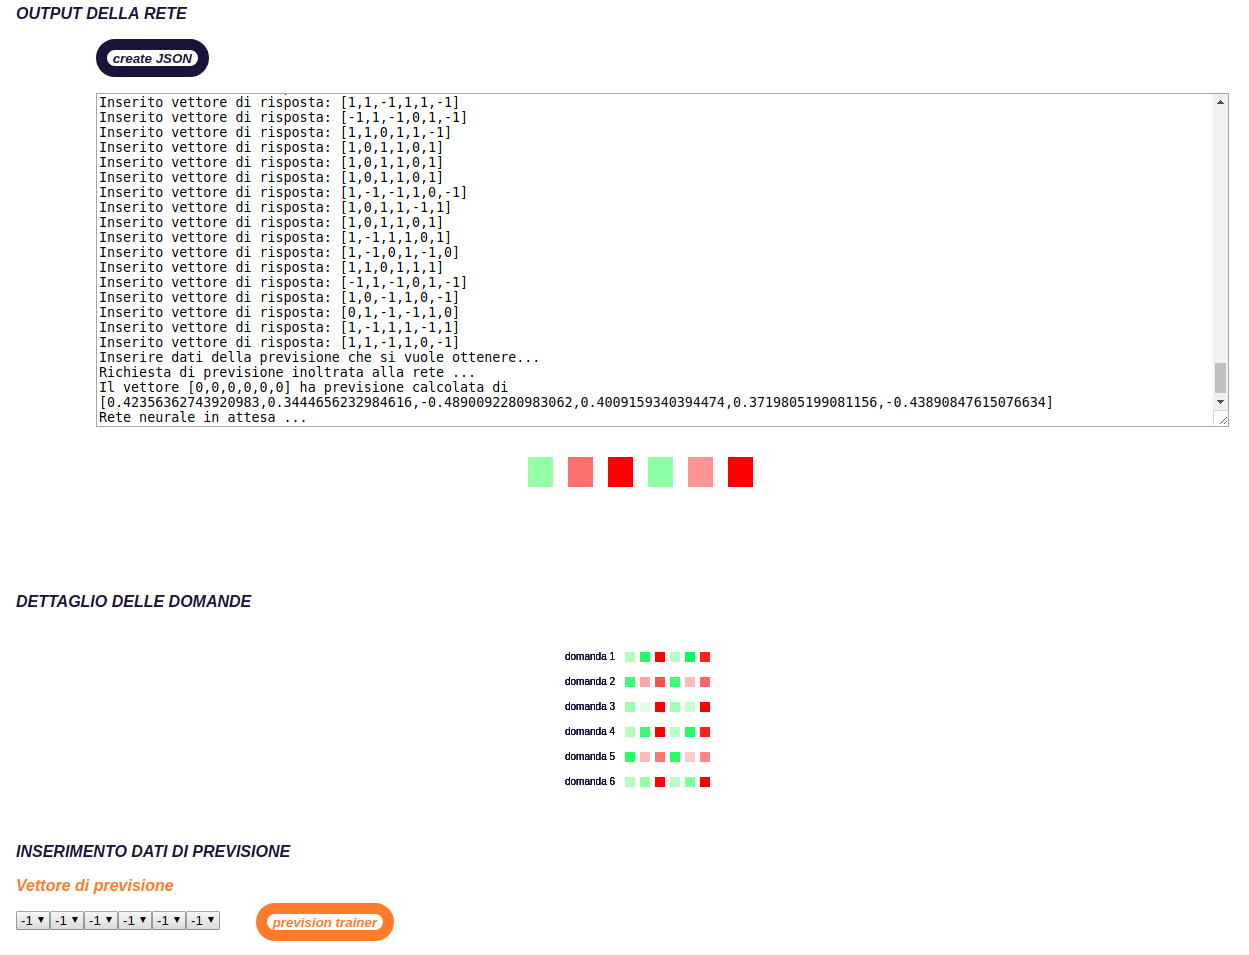
\includegraphics[width=0.90\linewidth]{./image/rete_prova-vpmeno1.png}
	\caption{Risultato della rete di prova a seguito di un vettore di previsione [-1, -1, -1, -1, -1, -1] in input.}
\end{figure}
\begin{itemize}
\item \textit{se la domanda 1 \`e settata a -1 (non corretta)}: la rete prevede che la domanda 1 e 4 non abbiano una probabilit\`a alta di essere risposte in modo corretto (bianco con sfumature di verde); la 3 e 6 una probabilit\`a molto alta di venire risposte in modo sbagliato (rosso), la 2 e la 5 di non venire nemmeno poste (verde con qualche sfumatura di bianco).
\item \textit{se la domanda 2 \`e settata a -1 (non corretta)}: la rete prevede che la domanda 1 e 4 abbiano una probabilit\`a non molto alta di essere risposte in modo non corretto (verde con qualche sfumatura di bianco); la 3 e 6 una buona probabilit\`a di venire risposte in modo sbagliato (rosa), la 2 e la 5 di venire date in modo non corretto (rosa molto atenuato).
\item \textit{se la domanda 3 \`e settata a -1 (non corretta)}: la rete prevede che la domanda 3 e 6 abbiano una probabilit\`a comunque alta di essere risposte in modo non corretto (rosso); la 1 e 4 con bassa probabilit\`a di venire risposte in modo corretto (bianco con qualche sfumatura di verde) perch\`e pi\`u semplici delle domande 3 e 6, la 2 e la 5 di non venire nemmeno poste o comunque basso di venire risposto correttamente(bianco con sfumature di verde).
\item \textit{se la domanda 4 \`e settata a -1 (non corretta)}: la rete prevede un risultato  identico a quanto ottenuto dalla domanda 1.
\item \textit{se la domanda 5 \`e settata a -1 (non corretta)}: la rete prevede un risultato similare a quanto ottenuto dalla domanda 2. Cambia solo quanto previsto dalle domande 3 e 6 che si presentano con un rosa un p\`o meno intenso, in quanto non  correlate alla coppia di domande 2 e 5.
\item \textit{se la domanda 6 \`e settata a -1 (non corretta)}: la rete prevede un risultato simile a quanto ottenuto dalla domanda 3. La coppia 2 e 5 hanno una probabilit\`a maggiore di essere date correttamente (bianco con sfumature di verde) ma perch\`e non correlate alle domande 3 e 6.
\end{itemize}
\end{itemize}

\paragraph{Test nella Rete del database}\mbox{}\\
\label{Test nella Rete del database}
\noindent
\subparagraph{Architetture testate}\mbox{}\\\\
\label{Architetture testate}
\noindent
Durante tutto il periodo ho effettuato una serie di test su molteplici architettura della rete, con gradi di correlazione tra le domande pari al 100\% o con uno differenza massima di 5 punti colore rispetto al canvas risultante per ogni domanda.\\
Tuttavia non sono riuscita ad individuare un'architettura sufficientemente stabile per prevedere risultati attendibili; a causa della molteplicit\`a di dati che hanno aumentato esponenzialmente  la complessit\`a di analisi rispetto alla Rete di prova, che non \`e calata neppure a seguito dell'analisi da parte mia delle domande presenti all'interno del database aziendale.
Architettura della rete utilizzata:
\begin{itemize}
\item \begin{verbatim}
layer_defs = [];
layer_defs.push({type:'input', out_sx:1, out_sy:1, out_depth:89});
layer_defs.push({type:'fc', num_neurons:2, activation: 'tanh'});
layer_defs.push({type:'fc', num_neurons:6, activation: 'tanh'});
layer_defs.push({type:'fc', num_neurons:4, activation: 'tanh'});
layer_defs.push({type:'regression', num_neurons:89});

net = new convnetjs.Net();
net.makeLayers(layer_defs);

trainer = new convnetjs.SGDTrainer(net, {learning_rate:0.01,
momentum:0.1, batch_size:10, l2_decay:0.001});
\end{verbatim}

\begin{figure}[H]
\centering
	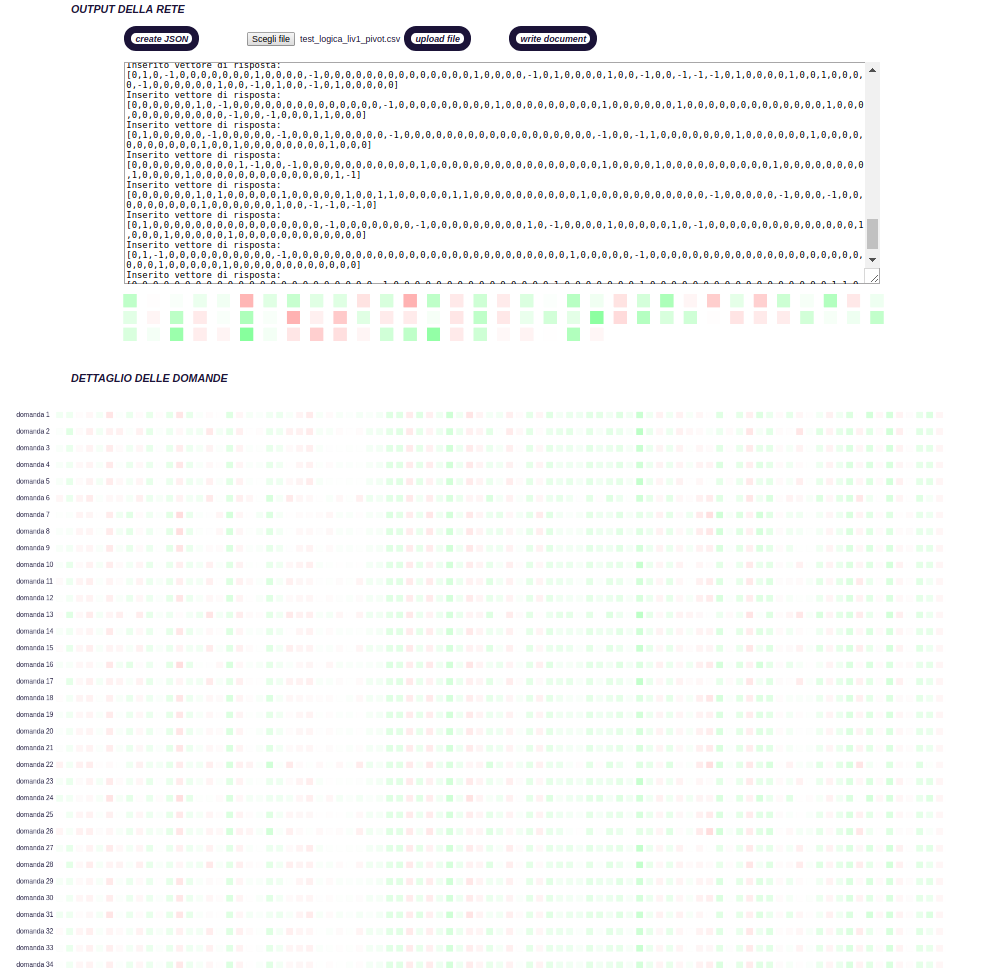
\includegraphics[width=0.90\linewidth]{./image/rete_db-vp1.png}
	\caption{Risultato della rete del database a seguito di un vettore di previsione [1, 1, 1, 1, 1, 1] in input.}
\end{figure}

\begin{figure}[H]
\centering
	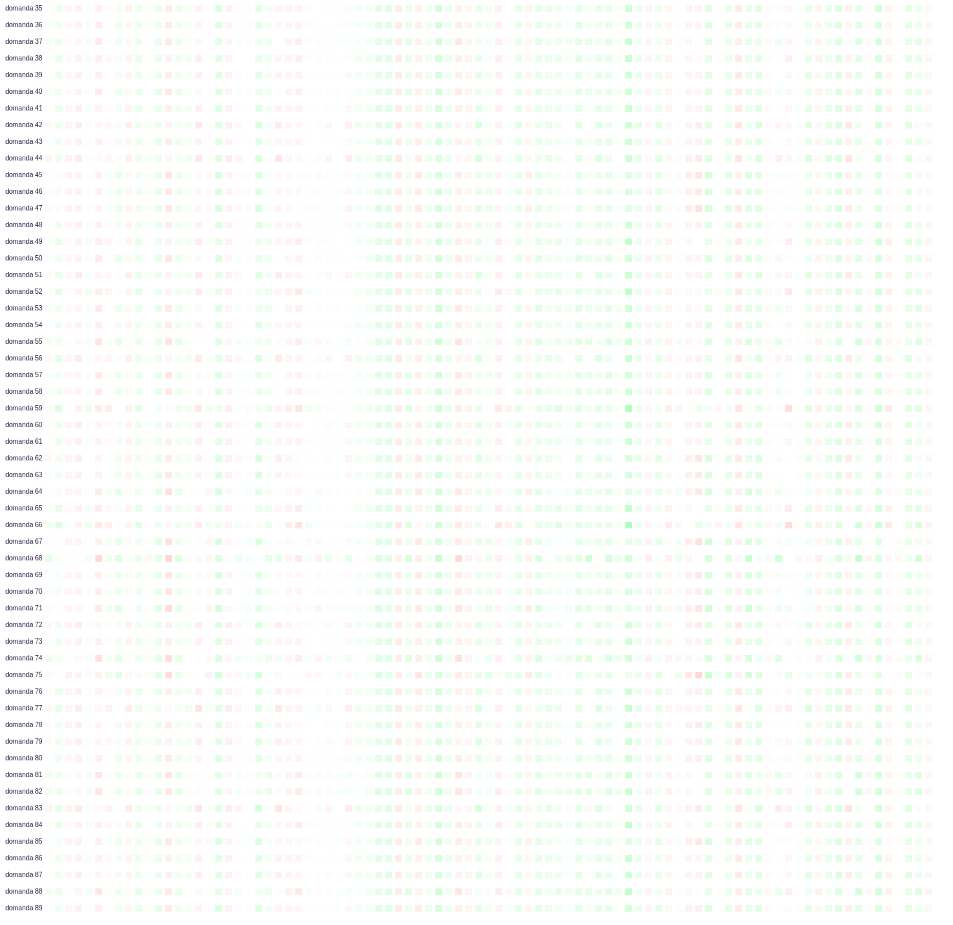
\includegraphics[width=0.90\linewidth]{./image/rete_db-vp1_2.png}
	\caption{Risultato della rete del database a seguito di un vettore di previsione [1, 1, 1, 1, 1, 1] in input.}
\end{figure}
\noindent
Dagli screen della rete riportati sopra appare come "sembrano" domande:
\begin{enumerate}
\item Analisi verticale:
\begin{itemize}
\item \textit{semplici} la 18, 22, 34, 35, 37, 39, 41, 44, 48, 50, 51, 52, 53, 54, 55, 56, 57, 59, 60, 67, 69,  71, 72, 77, 79, 80, 82, 84, 87 e 88. Inoltre di queste sembrano in relazione ancora pi\`u stretta le domande 18, 22, 40 e 59.
\item \textit{difficili} la 3, 4, 6, 13, 16, 19, 24, 25, 26, 36, 38, 42, 43, 46, 49, 61, 63, 65, 66, 70, 78, 81, 85 e 89. Inoltre di queste sembrano in relazione ancora pi\`u stretta le domande 6, 13, 19, 36, 38, 42, 46 e 70.
\end{itemize}
\item Analisi orizzontale:
Appaiono in relazione stretta le seguenti domande:
\begin{itemize}
\item 2, 3, 4, 5;
\item 7, 8, 9;
\item 14, 16;
\item 20, 21;
\item 26, 32;
\item 29, 32
\item 33, 34, 35, 36, 38;
\item 39, 41, 43;
\item 46, 48;
\item 49, 52;
\item 50, 53;
\item 72, 79;
\item 81, 82;
\item 86, 87, 88.
\end{itemize}
\end{enumerate}

\begin{figure}[H]
\centering
	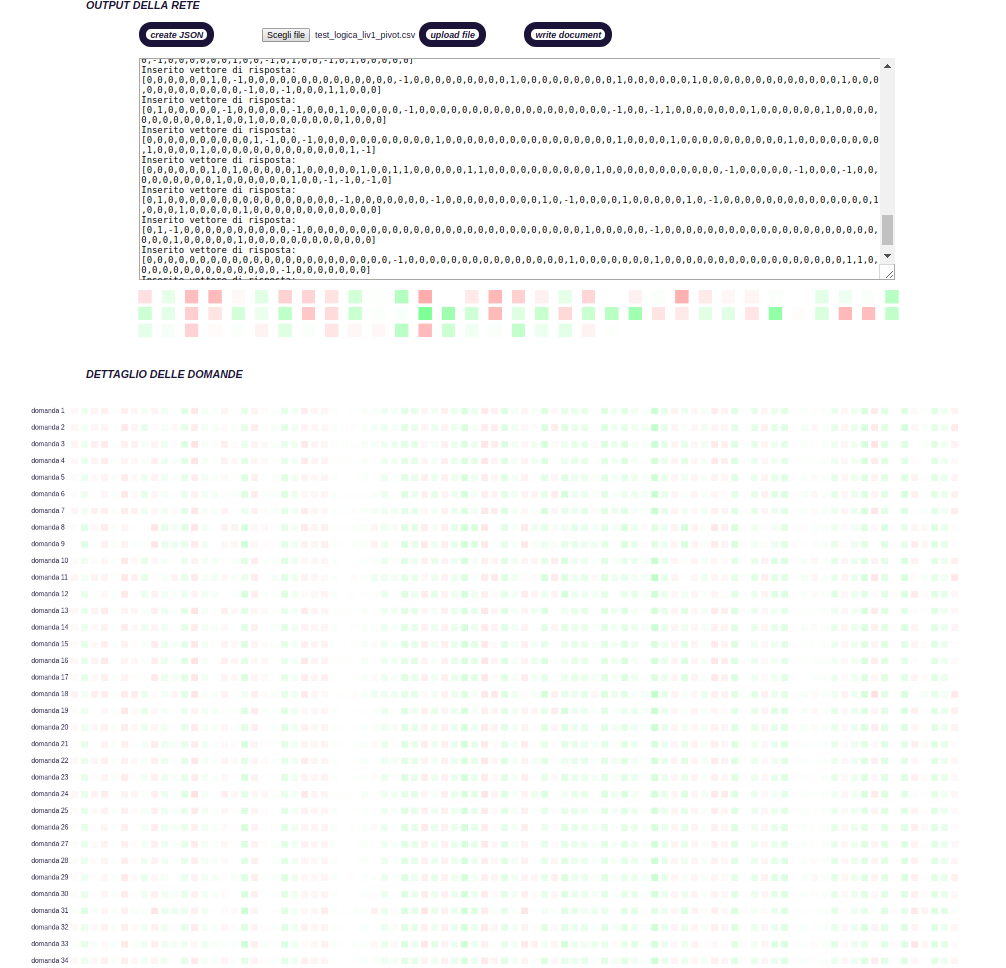
\includegraphics[width=0.90\linewidth]{./image/rete_db-vpmeno1.png}
	\caption{Risultato della rete del database a seguito di un vettore di previsione [-1, -1, -1, -1, -1, -1] in input.}
\end{figure}

\begin{figure}[H]
\centering
	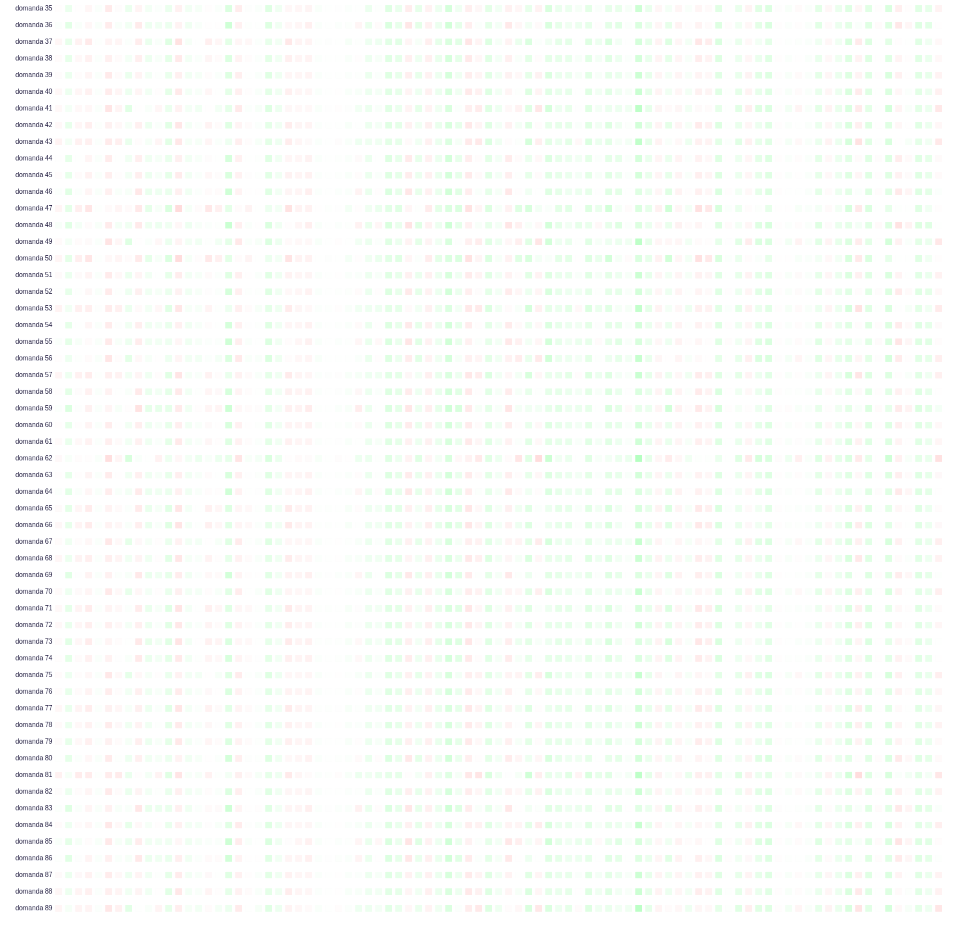
\includegraphics[width=0.90\linewidth]{./image/rete_db-vpmeno1_2.png}
	\caption{Risultato della rete del database a seguito di un vettore di previsione [-1, -1, -1, -1, -1, -1] in input.}
\end{figure}
\noindent
Dagli screen della rete riportati sopra appare come "sembrano" domande:
\begin{enumerate}
\item Analisi verticale:
\begin{itemize}
\item \textit{semplici} la 18, 22, 34, 35, 37, 38, 39, 41, 44, 48, 50, 51, 52, 54, 55, 56, 67, 69,  71, 72, 77, 79, 80, 82, 84, 87 e 88. Inoltre di queste sembrano in relazione ancora pi\`u stretta le domande 18, 22, 38, 52 e 57.
\item \textit{difficili} la 3, 4, 6, 13, 19, 27, 36, 38, 42, 43, 46, 61, 62, 65, 70. Inoltre di queste sembrano in relazione ancora pi\`u stretta le domande 6, 13, 19, 36, 38, 42, 46, 61 e 62.
\end{itemize}
\item Analisi orizzontale:
Appaiono in relazione stretta le seguenti domande:
\begin{itemize}
\item rimaste consistenti con il vettore [1, 1, 1, 1, 1, 1].
\end{itemize}
\end{enumerate}


\item \begin{verbatim}
layer_defs = [];
layer_defs.push({type:'input', out_sx:1, out_sy:1, out_depth:89});
layer_defs.push({type:'fc', num_neurons:12, activation: 'tanh'});
layer_defs.push({type:'regression', num_neurons:89});

net = new convnetjs.Net();
net.makeLayers(layer_defs);

trainer = new convnetjs.SGDTrainer(net, {learning_rate:0.01, momentum:0.1, batch_size:10, l2_decay:0.001});
\end{verbatim}
La prima cosa che ho notato \`e che aumentando il numero di neuroni sull'unico layer esistente, il valore della domanda corrispondente al vettore della previsione sembra sempre pi\`u marcato, segno che la rete "impara troppo" e ricade nel restituire l'immagine stessa del vettore previsione.

\begin{figure}[H]
\centering
	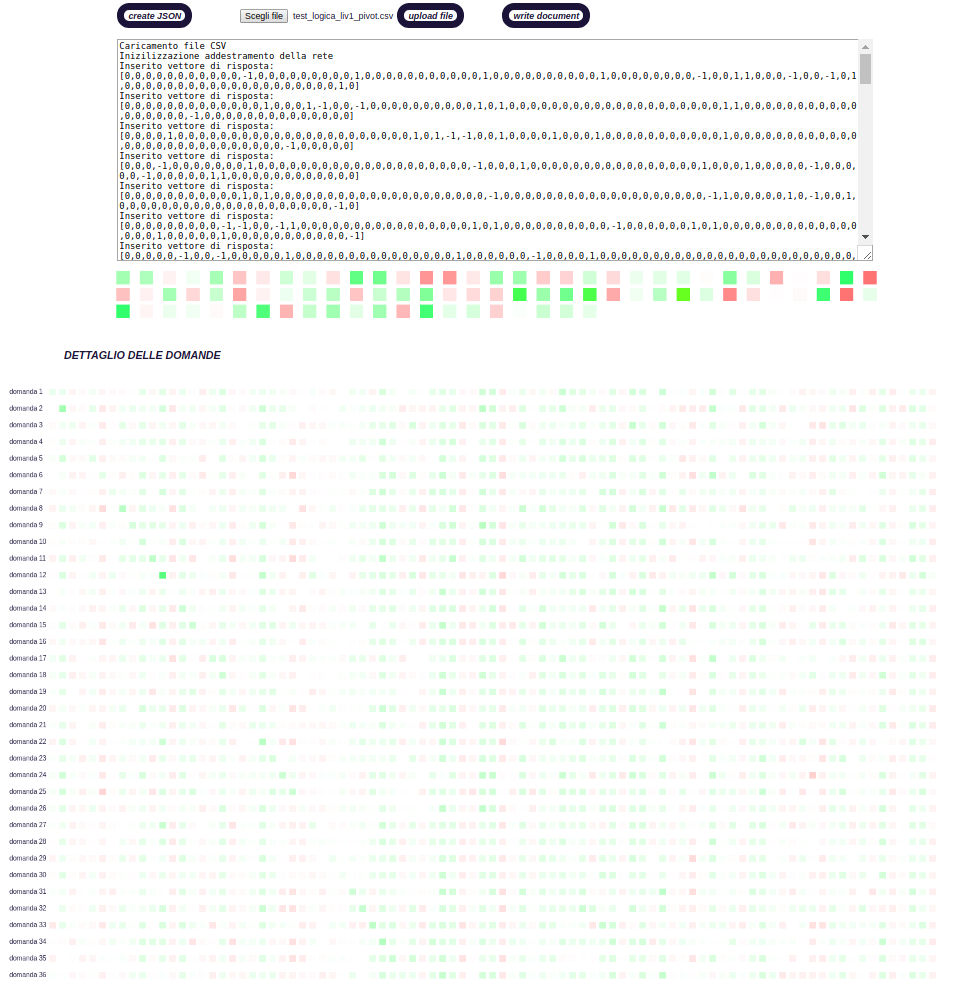
\includegraphics[width=0.90\linewidth]{./image/rete_db-vp1architettura2.png}
	\caption{Risultato della rete del database a seguito di un vettore di previsione [1, 1, 1, 1, 1, 1] in input.}
\end{figure}

\begin{figure}[H]
\centering
	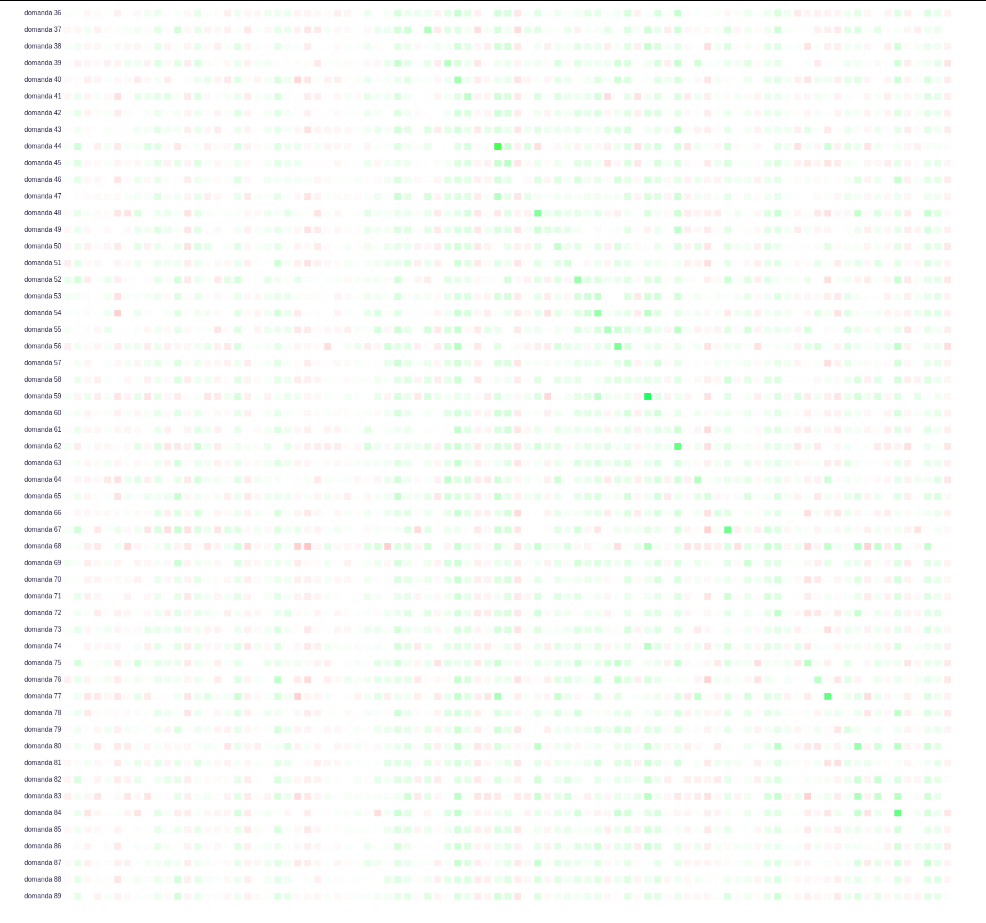
\includegraphics[width=0.90\linewidth]{./image/rete_db-vp1_2architettura2.png}
	\caption{Risultato della rete del database a seguito di un vettore di previsione [1, 1, 1, 1, 1, 1] in input.}
\end{figure}

Dagli screen della rete riportati sopra appare come la situazione appare meno lineare del caso analizzato precedentemente. 
Le domande non vengono separate per linee rete; ma per aree di relazione.


Dagli screen della rete riportati sopra appare come "sembrano" domande:
\begin{enumerate}
\item Analisi verticale:
\begin{itemize}
\item \textit{semplici} la 18, 22, 34, 35, 37, 39, 41, 44, 48, 50, 51, 52, 53, 54, 55, 56, 57, 59, 60, 67, 69,  71, 72, 77, 79, 80, 82, 84, 87 e 88. Inoltre di queste sembrano in relazione ancora pi\`u stretta le domande 18, 22, 40 e 59.
\item \textit{difficili} la 3, 4, 6, 13, 16, 19, 24, 25, 26, 36, 38, 42, 43, 46, 49, 61, 63, 65, 66, 70, 78, 81, 85 e 89. Inoltre di queste sembrano in relazione ancora pi\`u stretta le domande 6, 13, 19, 36, 38, 42, 46 e 70.
\end{itemize}
\item Analisi orizzontale:
Appaiono in relazione stretta le seguenti domande:
\begin{itemize}
\item Vengono meno le relazioni individuate precedentemente.
\end{itemize}
\end{enumerate}
\noindent


\item \begin{verbatim}
layer_defs = [];
layer_defs.push({type:'input', out_sx:1, out_sy:1, out_depth:89});
layer_defs.push({type:'fc', num_neurons:2, activation: 'tanh'});
layer_defs.push({type:'fc', num_neurons:6, activation: 'tanh'});
layer_defs.push({type:'fc', num_neurons:4, activation: 'tanh'});
layer_defs.push({type:'regression', num_neurons:89});

net = new convnetjs.Net();
net.makeLayers(layer_defs);

trainer = new convnetjs.SGDTrainer(net, {learning_rate:0.01,
momentum:0.1, batch_size:10, l2_decay:0.001});
\end{verbatim}

\item \begin{verbatim}
layer_defs = [];
layer_defs.push({type:'input', out_sx:1, out_sy:1, out_depth:89});
layer_defs.push({type:'fc', num_neurons:12, activation: 'tanh'});
layer_defs.push({type:'regression', num_neurons:89});

net = new convnetjs.Net();
net.makeLayers(layer_defs);

trainer = new convnetjs.SGDTrainer(net, {learning_rate:0.01,
momentum:0.1, batch_size:10, l2_decay:0.001});
\end{verbatim}

\item \begin{verbatim}
layer_defs = [];
layer_defs.push({type:'input', out_sx:1, out_sy:1, out_depth:89});
layer_defs.push({type:'fc', num_neurons:12, activation: 'tanh'});
layer_defs.push({type:'fc', num_neurons:8, activation: 'tanh'});
layer_defs.push({type:'fc', num_neurons:6, activation: 'tanh'});
layer_defs.push({type:'fc', num_neurons:4, activation: 'tanh'});
layer_defs.push({type:'regression', num_neurons:89});

net = new convnetjs.Net();
net.makeLayers(layer_defs);

trainer = new convnetjs.SGDTrainer(net, {learning_rate:0.01, 
momentum:0.1, batch_size:10, l2_decay:0.001});
\end{verbatim}



\item \begin{verbatim}
layer_defs = [];
layer_defs.push({type:'input', out_sx:1, out_sy:1, out_depth:89});
layer_defs.push({type:'fc', num_neurons:2, activation: 'tanh'});
layer_defs.push({type:'fc', num_neurons:6, activation: 'tanh'});
layer_defs.push({type:'fc', num_neurons:6, activation: 'tanh'});
layer_defs.push({type:'fc', num_neurons:4, activation: 'tanh'});
layer_defs.push({type:'regression', num_neurons:89});

net = new convnetjs.Net();
net.makeLayers(layer_defs);

trainer = new convnetjs.SGDTrainer(net, {learning_rate:0.01, 
momentum:0.1, batch_size:10, l2_decay:0.001})
\end{verbatim}



\item \begin{verbatim}
layer_defs = [];
layer_defs.push
({type:'input', out_sx:1, out_sy:1, out_depth:89});
layer_defs.push({type:'fc', num_neurons:2, activation: 'tanh'});
layer_defs.push({type:'fc', num_neurons:4, activation: 'tanh'});
layer_defs.push({type:'fc', num_neurons:6, activation: 'tanh'});
layer_defs.push({type:'fc', num_neurons:4, activation: 'tanh'});
layer_defs.push({type:'regression', num_neurons:89});

net = new convnetjs.Net();
net.makeLayers(layer_defs);

trainer = new convnetjs.SGDTrainer(net, {learning_rate:0.01, 
momentum:0.1, batch_size:10, l2_decay:0.001});
\end{verbatim}


\item \begin{verbatim}
layer_defs = [];
layer_defs.push({type:'input', out_sx:1, out_sy:1, out_depth:89});
layer_defs.push({type:'fc', num_neurons:2, activation: 'tanh'});
layer_defs.push({type:'fc', num_neurons:6, activation: 'tanh'});
layer_defs.push({type:'fc', num_neurons:2, activation: 'tanh'});
layer_defs.push({type:'regression', num_neurons:89});

net = new convnetjs.Net();
net.makeLayers(layer_defs);

trainer = new convnetjs.SGDTrainer(net, {learning_rate:0.01, 
momentum:0.1, batch_size:10, l2_decay:0.001});
\end{verbatim}


\item \begin{verbatim}
layer_defs = [];
layer_defs.push({type:'input', out_sx:1, out_sy:1, out_depth:89});
layer_defs.push({type:'fc', num_neurons:2, activation: 'tanh'});
layer_defs.push({type:'fc', num_neurons:4, activation: 'tanh'});
layer_defs.push({type:'fc', num_neurons:2, activation: 'tanh'});
layer_defs.push({type:'regression', num_neurons:89});

net = new convnetjs.Net();
net.makeLayers(layer_defs);

trainer = new convnetjs.SGDTrainer(net, {learning_rate:0.01, 
momentum:0.1, batch_size:10, l2_decay:0.001});
\end{verbatim}


\item \begin{verbatim}
layer_defs = [];
layer_defs.push({type:'input', out_sx:1, out_sy:1, out_depth:89});
layer_defs.push({type:'fc', num_neurons:2, activation: 'tanh'});
layer_defs.push({type:'fc', num_neurons:2, activation: 'tanh'});
layer_defs.push({type:'regression', num_neurons:89});

net = new convnetjs.Net();
net.makeLayers(layer_defs);

trainer = new convnetjs.SGDTrainer(net, {learning_rate:0.01, 
momentum:0.1, batch_size:10, l2_decay:0.001});
\end{verbatim}

\item \begin{verbatim}
layer_defs = [];
layer_defs.push({type:'input', out_sx:1, out_sy:1, out_depth:89});
layer_defs.push({type:'fc', num_neurons:4, activation: 'tanh'});
layer_defs.push({type:'fc', num_neurons:4, activation: 'tanh'});
layer_defs.push({type:'regression', num_neurons:89});

net = new convnetjs.Net();
net.makeLayers(layer_defs);

trainer = new convnetjs.SGDTrainer(net, {learning_rate:0.01, 
momentum:0.1, batch_size:10, l2_decay:0.001});
\end{verbatim}


\item \begin{verbatim}
layer_defs = [];
layer_defs.push({type:'input', out_sx:1, out_sy:1, out_depth:89});
layer_defs.push({type:'fc', num_neurons:3, activation: 'tanh'});
layer_defs.push({type:'fc', num_neurons:3, activation: 'tanh'});
layer_defs.push({type:'regression', num_neurons:89});

net = new convnetjs.Net();
net.makeLayers(layer_defs);

trainer = new convnetjs.SGDTrainer(net, {learning_rate:0.01,
 momentum:0.1, batch_size:10, l2_decay:0.001});
\end{verbatim}


\item \begin{verbatim}
layer_defs = [];
layer_defs.push({type:'input', out_sx:1, out_sy:1, out_depth:89});
layer_defs.push({type:'fc', num_neurons:3, activation: 'tanh'});
layer_defs.push({type:'fc', num_neurons:2, activation: 'tanh'});
layer_defs.push({type:'regression', num_neurons:89});

net = new convnetjs.Net();
net.makeLayers(layer_defs);

trainer = new convnetjs.SGDTrainer(net, {learning_rate:0.01, 
momentum:0.1, batch_size:10, l2_decay:0.001});
\end{verbatim}


\item \begin{verbatim}
layer_defs = [];
layer_defs.push({type:'input', out_sx:1, out_sy:1, out_depth:89});
layer_defs.push({type:'fc', num_neurons:2, activation: 'tanh'});
layer_defs.push({type:'fc', num_neurons:3, activation: 'tanh'});
layer_defs.push({type:'fc', num_neurons:1, activation: 'tanh'});
layer_defs.push({type:'regression', num_neurons:89});

net = new convnetjs.Net();
net.makeLayers(layer_defs);

trainer = new convnetjs.SGDTrainer(net, {learning_rate:0.01, 
momentum:0.1, batch_size:10, l2_decay:0.001});
\end{verbatim}


\item \begin{verbatim}
layer_defs = [];
layer_defs.push({type:'input', out_sx:1, out_sy:1, out_depth:89});
layer_defs.push({type:'fc', num_neurons:2, activation: 'tanh'});
layer_defs.push({type:'fc', num_neurons:3, activation: 'tanh'});
layer_defs.push({type:'fc', num_neurons:2, activation: 'tanh'});
layer_defs.push({type:'regression', num_neurons:89});

net = new convnetjs.Net();
net.makeLayers(layer_defs);

trainer = new convnetjs.SGDTrainer(net, {learning_rate:0.01, 
momentum:0.1, batch_size:10, l2_decay:0.001});
\end{verbatim}


\item \begin{verbatim}
layer_defs = [];
layer_defs.push({type:'input', out_sx:1, out_sy:1, out_depth:89});
layer_defs.push({type:'fc', num_neurons:2, activation: 'tanh'});
layer_defs.push({type:'fc', num_neurons:4, activation: 'tanh'});
layer_defs.push({type:'fc', num_neurons:1, activation: 'tanh'});
layer_defs.push({type:'regression', num_neurons:89});

net = new convnetjs.Net();
net.makeLayers(layer_defs);

trainer = new convnetjs.SGDTrainer(net, {learning_rate:0.01, 
momentum:0.1, batch_size:10, l2_decay:0.001});
\end{verbatim}

\item \begin{verbatim}
layer_defs = [];
layer_defs.push({type:'input', out_sx:1, out_sy:1, out_depth:89});
layer_defs.push({type:'fc', num_neurons:2, activation: 'tanh'});
layer_defs.push({type:'fc', num_neurons:5, activation: 'tanh'});
layer_defs.push({type:'fc', num_neurons:1, activation: 'tanh'});
layer_defs.push({type:'regression', num_neurons:89});

net = new convnetjs.Net();
net.makeLayers(layer_defs);

trainer = new convnetjs.SGDTrainer(net, {learning_rate:0.01,
momentum:0.1, batch_size:10, l2_decay:0.001});
\end{verbatim}


\item \begin{verbatim}
layer_defs = [];
layer_defs.push({type:'input', out_sx:1, out_sy:1, out_depth:89});
layer_defs.push({type:'fc', num_neurons:1, activation: 'tanh'});
layer_defs.push({type:'fc', num_neurons:4, activation: 'tanh'});
layer_defs.push({type:'fc', num_neurons:1, activation: 'tanh'});
layer_defs.push({type:'regression', num_neurons:89});

net = new convnetjs.Net();
net.makeLayers(layer_defs);

trainer = new convnetjs.SGDTrainer(net, {learning_rate:0.01, 
momentum:0.1, batch_size:10, l2_decay:0.001});
\end{verbatim}

\item \begin{verbatim}
layer_defs = [];
layer_defs.push({type:'input', out_sx:1, out_sy:1, out_depth:89});
layer_defs.push({type:'fc', num_neurons:3, activation: 'tanh'});
layer_defs.push({type:'fc', num_neurons:4, activation: 'tanh'});
layer_defs.push({type:'fc', num_neurons:1, activation: 'tanh'});
layer_defs.push({type:'regression', num_neurons:89});

net = new convnetjs.Net();
net.makeLayers(layer_defs);

trainer = new convnetjs.SGDTrainer(net, {learning_rate:0.01, 
momentum:0.1, batch_size:10, l2_decay:0.001});
\end{verbatim}


\item \begin{verbatim}
layer_defs = [];
layer_defs.push({type:'input', out_sx:1, out_sy:1, out_depth:89});
layer_defs.push({type:'fc', num_neurons:6, activation: 'tanh'});
layer_defs.push({type:'fc', num_neurons:6, activation: 'tanh'});
layer_defs.push({type:'fc', num_neurons:6, activation: 'tanh'});
layer_defs.push({type:'fc', num_neurons:6, activation: 'tanh'});
layer_defs.push({type:'regression', num_neurons:89});

net = new convnetjs.Net();
net.makeLayers(layer_defs);

trainer = new convnetjs.SGDTrainer(net, {learning_rate:0.01, 
momentum:0.1, batch_size:10, l2_decay:0.001});
\end{verbatim}

\item \begin{verbatim}
layer_defs = [];
layer_defs.push({type:'input', out_sx:1, out_sy:1, out_depth:89});
layer_defs.push({type:'fc', num_neurons:18, activation: 'tanh'});
layer_defs.push({type:'fc', num_neurons:18, activation: 'tanh'});
layer_defs.push({type:'regression', num_neurons:89});

net = new convnetjs.Net();
net.makeLayers(layer_defs);

trainer = new convnetjs.SGDTrainer(net, {learning_rate:0.01, 
momentum:0.1, batch_size:10, l2_decay:0.001});
\end{verbatim}

\item \begin{verbatim}
layer_defs = [];
layer_defs.push({type:'input', out_sx:1, out_sy:1, out_depth:89});
layer_defs.push({type:'fc', num_neurons:18, activation: 'tanh'});
layer_defs.push({type:'fc', num_neurons:18, activation: 'tanh'});
layer_defs.push({type:'fc', num_neurons:18, activation: 'tanh'});
layer_defs.push({type:'regression', num_neurons:89});

net = new convnetjs.Net();
net.makeLayers(layer_defs);

trainer = new convnetjs.SGDTrainer(net, {learning_rate:0.01, 
momentum:0.1, batch_size:10, l2_decay:0.001});
\end{verbatim}

\item \begin{verbatim}
layer_defs = [];
layer_defs.push({type:'input', out_sx:1, out_sy:1, out_depth:89});
layer_defs.push({type:'fc', num_neurons:2, activation: 'tanh'});
layer_defs.push({type:'fc', num_neurons:3, activation: 'tanh'});
layer_defs.push({type:'fc', num_neurons:2, activation: 'tanh'});
layer_defs.push({type:'fc', num_neurons:1, activation: 'tanh'});
layer_defs.push({type:'regression', num_neurons:89});

net = new convnetjs.Net();
net.makeLayers(layer_defs);

trainer = new convnetjs.SGDTrainer(net, {learning_rate:0.01,
 momentum:0.1, batch_size:10, l2_decay:0.001});
\end{verbatim}

\item \begin{verbatim}
layer_defs = [];
layer_defs.push({type:'input', out_sx:1, out_sy:1, out_depth:89});
layer_defs.push({type:'fc', num_neurons:2, activation: 'tanh'});
layer_defs.push({type:'fc', num_neurons:3, activation: 'tanh'});
layer_defs.push({type:'fc', num_neurons:3, activation: 'tanh'});
layer_defs.push({type:'fc', num_neurons:1, activation: 'tanh'});
layer_defs.push({type:'regression', num_neurons:89});

net = new convnetjs.Net();
net.makeLayers(layer_defs);

trainer = new convnetjs.SGDTrainer(net, {learning_rate:0.01, 
momentum:0.1, batch_size:10, l2_decay:0.001});
\end{verbatim}

\item \begin{verbatim}
layer_defs = [];
layer_defs.push({type:'input', out_sx:1, out_sy:1, out_depth:89});
layer_defs.push({type:'fc', num_neurons:2, activation: 'tanh'});
layer_defs.push({type:'fc', num_neurons:6, activation: 'tanh'});
layer_defs.push({type:'fc', num_neurons:3, activation: 'tanh'});
layer_defs.push({type:'fc', num_neurons:1, activation: 'tanh'});
layer_defs.push({type:'regression', num_neurons:89});

net = new convnetjs.Net();
net.makeLayers(layer_defs);

trainer = new convnetjs.SGDTrainer(net, {learning_rate:0.01, 
momentum:0.1, batch_size:10, l2_decay:0.001});
\end{verbatim}

\item \begin{verbatim}
layer_defs = [];
layer_defs.push({type:'input', out_sx:1, out_sy:1, out_depth:89});
layer_defs.push({type:'fc', num_neurons:2, activation: 'tanh'});
layer_defs.push({type:'fc', num_neurons:6, activation: 'tanh'});
layer_defs.push({type:'fc', num_neurons:4, activation: 'tanh'});
layer_defs.push({type:'fc', num_neurons:1, activation: 'tanh'});
layer_defs.push({type:'regression', num_neurons:89});

net = new convnetjs.Net();
net.makeLayers(layer_defs);

trainer = new convnetjs.SGDTrainer(net, {learning_rate:0.01, 
momentum:0.1, batch_size:10, l2_decay:0.001});
\end{verbatim}


\item \begin{verbatim}
layer_defs = [];
layer_defs.push({type:'input', out_sx:1, out_sy:1, out_depth:89});
layer_defs.push({type:'fc', num_neurons:8, activation: 'tanh'});
layer_defs.push({type:'fc', num_neurons:8, activation: 'tanh'});
layer_defs.push({type:'regression', num_neurons:89});

net = new convnetjs.Net();
net.makeLayers(layer_defs);

trainer = new convnetjs.SGDTrainer(net, {learning_rate:0.01, 
momentum:0.1, batch_size:10, l2_decay:0.001});
\end{verbatim}
\end{itemize}\pagebreak
\section{Principal Component Analysis}
\label{PCA}

La \textbf{P}rincipal \textbf{C}omponent \textbf{A}nalysis (acronimo PCA) \`e una tecnica impiegata nell'ambito della statistica multivariata\footnote{parte della statistica in cui l'oggetto dell'analisi \`e almeno composta da due elementi} usata per semplificare i dati d'origine.\\
Lo scopo che tale tecnica persegue \`e lo studio della relazione esistenti tra i campioni d'interesse, con la riduzione di un numero pi\`u o meno elevato di variabili. La riduzione dimensionale avviene tramite una trasformazione lineare delle variabili coinvolte con lo scopo di effettuare la proiezione di quelle originarie in un nuovo sistema cartesiano, in cui tutte le variabili vengono ordinate in maniera decrescente per ordine di varianza. Successivamente la variabile con maggiore varianza viene proiettata sul primo asse, la seconda sul secondo e via via sempre cos\`i per tutte le variabili sotto esame. La PCA \`	e particolarmente utile quando la dimensionalit\`a dello spazio delle misure \`e elevata (molte colonne); tuttavia i campioni si vengono a trovare in uno spazio di dimensioni significativamente ridotte.\\
Indispensabile per la buona riuscita della tecnica \`e, come gi\`a esposto sopra, la ricerca del numero di componenti principali significative, ovvero tutte le variabili coinvolte a meno di quelle legate al rumore, che concorrono a comporre la \textit{dimensionalit\`a intrinseca}. Il "rumore" \`e sempre concentrato nelle ultime variabili, non includerle nell'analisi dei dati porta a dati pi\`u puliti, con un rapporto segnale/rumore pi\`u alto.\\
Il calcolo di quali sono le componenti pi\`u significative si ottiene con la varianza. La prima componente principale spiega la massima percentuale della variabilit\`a presente nei dati rappresentabili in una singola dimensione, in poche parole la direzione lungo cui si registra la massima dispersione dei dati (quanto il valore medio si discosta). La varianza porta il vantaggio di essere indipendente dal sistema di riferimento, difatti conseguentemente una rotazione degli assi mantiene immutata la varianza totale all'interno del sistema.

\subsection{Metodologia applicata}
\label{Metodologia applicata}
L'analisi e l'implementazione della tecnica di \textbf{P}rincipal \textbf{C}omponent \textbf{A}nalysis l'ho svolta nel periodo 17 - 21 luglio con la seguente metodologia:
\begin{itemize}
\item Studio e configurazione di R e R-Studio;
\item Studio del significato della tecnica e sua correlazione con le Rete neurali;
\item Studio della metodologia di implementazione;
\item Scelta del package pi\`u adeguato per svolgere l'applicazione della PCA sui dati di trainset;
\item Implementazione del metodo della PCA  e dei metodi di supporto ad analisi dei dati.
\item Analisi dei risultati ottenuti dalla PCA;
\item Analisi delle domande presenti nel database aziendale;
\item Confronto dei risultati della PCA con quelli ottenuti dalla Rete neurale e confronto della loro validit\`a con le domande del database.
\end{itemize}
\noindent
Ogni implementazione  e osservazione l'ho svolta prima nei dati del trainset di prova e solo successivamente gli traslati all'interno del trainset delle domande nel database aziendale. In modo ho avuto sempre ben la correttezza e le possibili correlazioni vigenti nel metodo in uso.

\subsection{Sviluppo}
\label{Sviluppo}
La tecnica di PCA effettua analisi dei dati. I dati che ho impiegato sono i medesimi che ho utilizzato per effettuare il trainset della Rete neurale. Il formato utilizzato \`e sempre CSV e i dati contenuti sono strutturati per riga con  i risultati di ogni test e per colonna con il risultato di una specifica domanda k.
\begin{enumerate}
\item Caricamento del package \textbf{factoextra}: la mia scelta \`e ricaduta su tale package e non in altri con la medesima funzione, per via della sua  visualizzazione dei dati elegante basata su ggplot2;
\item \textbf{Caricamento del file CSV} in memoria per mezzo della trasposizione in ata frame;
\item \textit{Standardizzazione} dei dati del trainset. Tale compito mi \`e risultato indispensabile  perch\`e anche se di norma, la standardizzazione, viene usata per evitare situazioni erronee (alcune variabili X presentate con una variabilit\`a molto maggiore rispetto ad altre) e io nei casi in analisi ero in possesso di dati gi\`a presentati con la medesima scala;  avendo la necessit\`a di individuare gli autovettori e  applicare il criterio di Keiser nel trainset ho dovuto procedere ugualmente a standardizzare.
\item Calcolo della \textbf{PCA} con la seguente formula:
\begin{verbatim}
prcomp(df_numeric, scale = FALSE) 
\end{verbatim}
R offre due metodi per calcolare la PCA: 
\begin{itemize}
\item \textit{prcomp(x, scale = FALSE)}: dove \textit{x} rappresenta una matrice numerica o data frame e \textit{scale} un valore logico che indica se le variabili devono essere ridimensionate/standardizzate;
\item \textit{princomp(x, cor = FALSE, scores = TRUE)}: dove \textit{x} rappresenta una matrice numerica o data frame, \textit{cor} valore logico che se a true ridimensiona e centra i dati prima di procedere all'analisi e \textit{scores} valore logico che se a true calcola le coordinate su ciascun componente principale.\\
Metodologia che ho utilizzato per passi:
\end{itemize}
\noindent
 Ho deciso di far uso della funzione \textit{prcomp} perch\`e usa la decomposizione del valore singolare (SGV) che offre una precisione leggermente migliore rispetto all'uso del metodo princomp.
 Il metodo \textit{prcomp} include nei propri elementi di output:
 \begin{enumerate}
 \item sdev: deviazione standard delle componenti principali;
 \item rotation: la matrice dei carichi delle variabili ovvero le colonne degli autovettori;
 \item center: la media variabile, indica se le variabili devono essere spostate per essere centrate sullo zero;
 \item scale: deviazione standard delle variabili;
 \item x: coordinate degli individui sulle componenti principali.
 \end{enumerate}
 \noindent
\item Calcolo degli \textbf{autovalori della matrice di covarianza}. Mostra la percentuale di varianze di competenza di ciascun componente principale con
\begin{verbatim}
get_eig(res.pca)
\end{verbatim}

\item \textbf{Riepilogo} mediante il metodo summary dei risultati ottenuti dal calcolo della PCA. Effettua la standardizzazione dei risultati ottenuti e ne calcola gli autovalori di covarianza con individuazione di deviazione standard, proporzione della varianza e proporzione cumulata.
\begin{verbatim}
summary(res.pca)
\end{verbatim}
\item \textbf{Calcolo degli autovettori} con
\begin{verbatim}
loadings(res.pca)
\end{verbatim}

\item \textbf{Individuazione della matrice correlazione} dei dati con
\begin{verbatim}
cor(df_numeric)
\end{verbatim}

\item Creazione di un data frame contenete per ogni variabile principale quali sono le componenti ordinate in modo decrescente strettamente correlate.
\end{enumerate}

\subsection{Risultati ottenuti}
\label{Risultati ottenuti}

\textit{I dati risultati dall'elaborazione dei dati inerenti il trainset delle domande nel database gli ho riportati, per motivi di spazio e comprensione, in modo parziale. Ogni metodo utilizzato viene di seguito descritto nel dettaglio.}

\subsubsection{Calcolo della Principal Component Analysis}
\label{Calcolo della Principal Component Analysis}
\begin{figure}[H]
\centering
	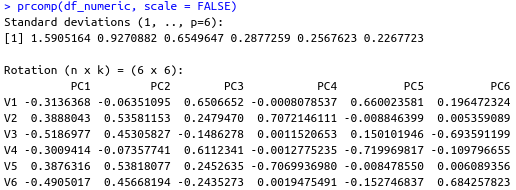
\includegraphics[width=0.80\linewidth]{../../PCA/plot/prcomp_rete-prova.png}
	\caption{Visualizzazione del calcolo della PCA tramite prcomop per il trainset di prova.}
\end{figure}

\begin{figure}[H]
\centering
	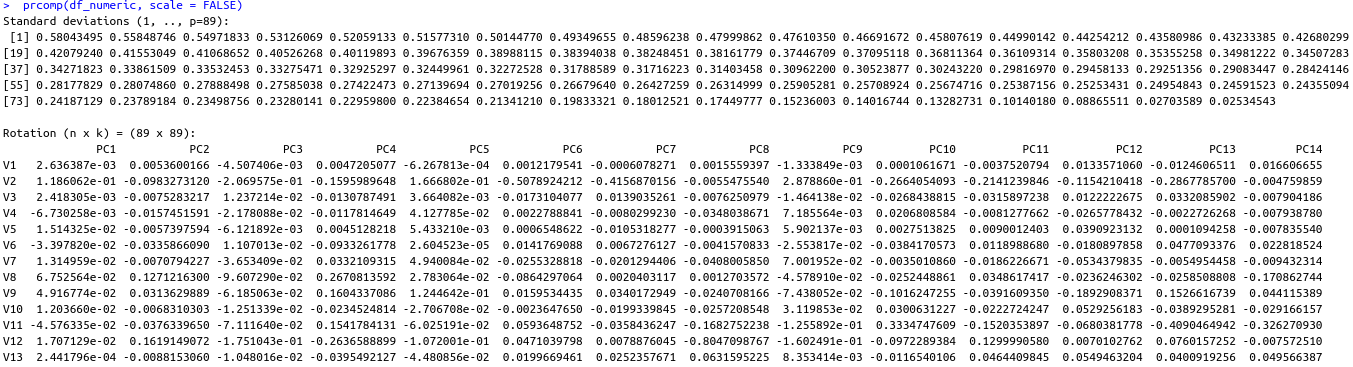
\includegraphics[width=1\linewidth]{../../PCA/plot/prcomp_rete-db.png}
	\caption{Visualizzazione del calcolo della PCA tramite prcomop per il trainset delle domande nel database.}
\end{figure}
\noindent

\paragraph{Osservazioni}
Osservando  esclusivamente la deviazione standard ottenuta dal trainset di prova, appare come i PC da prendere in considerazione per l'analisi sono i primi tre; inoltre  nella rotazione appare chiaro ch le valutazioni ottenute da V1 sono in relazione con V4, V3 con V6 e V2 con V5. Tuttavia queste sono solo mere osservazioni senza ancora alcuna prova matematica  completa a supporto. \\\\ Per quanto concerne il trainset delle domande nel database \`e molto difficile fare qualunque tipo di assunzione sulla natura dei dati causa la loro numerosit\`a.

\subsubsection{Calcolo degli autovettori ed individuazione di Summary}
\label{Calcolo degli autovettori ed individuazione di Summary}
\begin{figure}[H]
\centering
	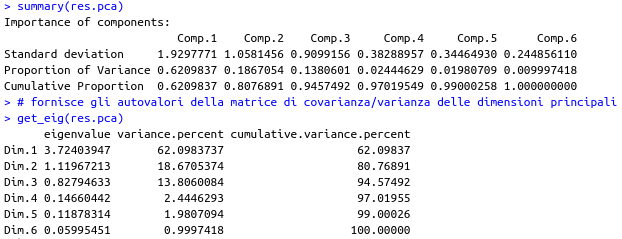
\includegraphics[width=0.80\linewidth]{../../PCA/plot/summary-autovalore_rete-prova.png}
	\caption{Visualizzazione del calcolo del metodo summary ed individuazione degli autovalori per il trainset di prova.}
\end{figure}
\begin{figure}[H]
\centering
	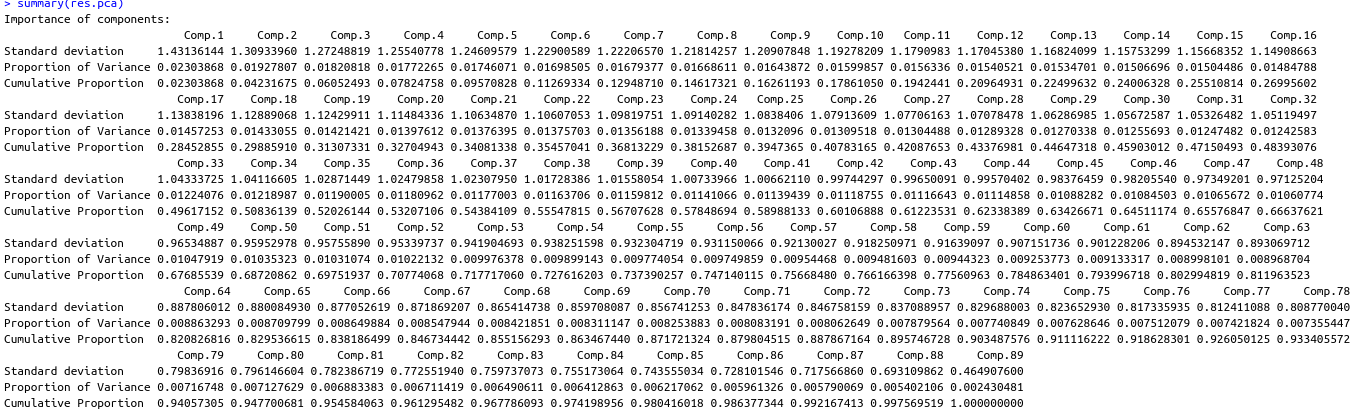
\includegraphics[width=1\linewidth]{../../PCA/plot/summary_db.png}
	\caption{Visualizzazione del calcolo del metodo summary per il trainset delle domande nel database.}
\end{figure}
\begin{figure}[H]
\centering
	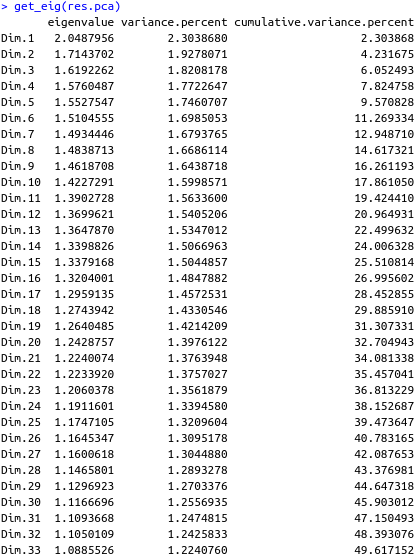
\includegraphics[width=0.60\linewidth]{../../PCA/plot/autovalori_db.png}
	\caption{Individuazione degli autovalori per il trainset delle domande nel database.}
\end{figure}
\paragraph{Osservazioni}
\`E essenziale per individuare il numero di componenti (PC) necessarie per effettuare un'analisi corretta basarsi sul calcolo della \textit{variance.percent} o \textit{Proportion of Variance}. A tale scopo \`e prendere le componenti principali che catturano la maggior parte di variabilti\`a dei dati.\\
Nel caso del trainset di prova basta le variabili PC1, PC2 e PC3 sono sufficienti a catturare il ~93\% della variabilit\`a presente.\\
Quanto appena descritto si pu\`o riscontrare anche graficamente, come presentato di seguito.

\begin{figure}[H]
\centering
	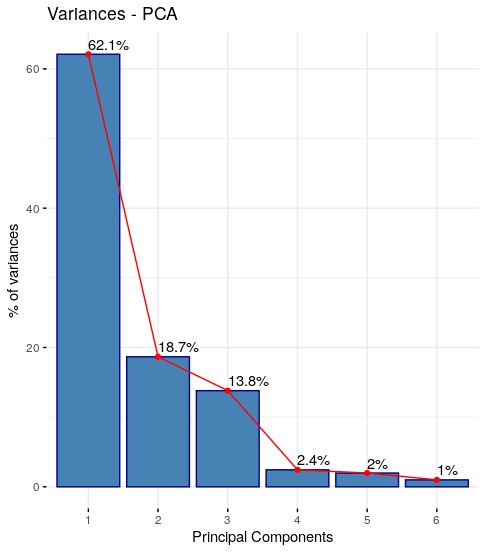
\includegraphics[width=0.60\linewidth]{../../PCA/plot/variances_rete-prova.png}
	\caption{Plot della rappresentazione grafica della varianza sui PC del trainset di prova.}
\end{figure}

\begin{figure}[H]
\centering
	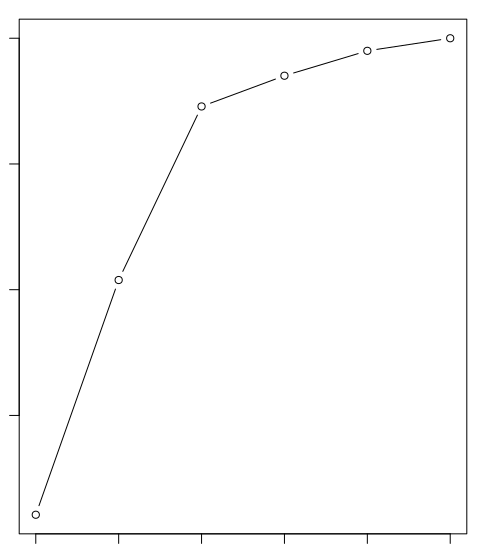
\includegraphics[width=0.60\linewidth]{../../PCA/plot/variances2_rete-prova.png}
	\caption{Plot della rappresentazione grafica della varianza sui PC del trainset di prova.}
\end{figure}
\noindent
Le ultime PC4, PC5 e PC6 hanno una variabilit\`a molto bassa, trascurabile.
\begin{figure}[H]
\centering
	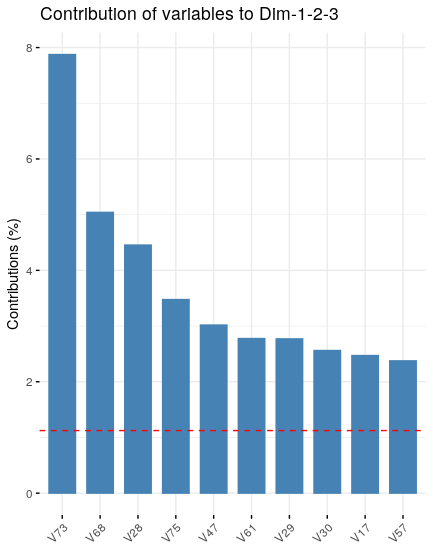
\includegraphics[width=0.60\linewidth]{../../PCA/plot/varianza-complessiva_rete-prova.png}
	\caption{Rappresentazione grafica di come la varianza si distribuisce sulle PC individuate dal modello sul trainset di prova.}
\end{figure}
\noindent
Tuttavia per quanto riguarda le domande nel database ogni conclusione "a occhio " risulta  impossibile da effettuare sempre a causa della numerosit\`a dei dati di trainset. L'utilizzo di un analisi dei risultati per mezzo di plot \`e l'unica via percorribile.

\begin{figure}[H]
\centering
	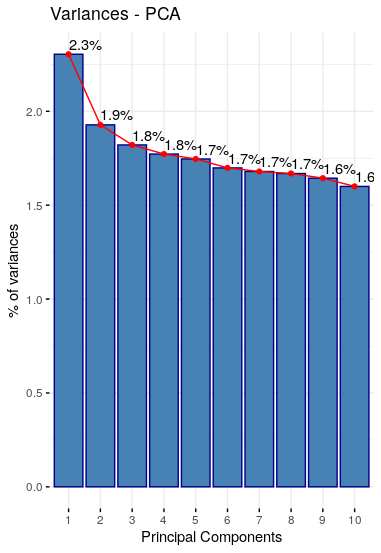
\includegraphics[width=0.60\linewidth]{../../PCA/plot/variances_rete-db.png}
	\caption{Plot della rappresentazione grafica della varianza dei primi dieci PC del trainset delle domande nel database.}
\end{figure}
\noindent
Il plot mostra esclusivamente le prime dieci componenti; tutte si presentano con una varianza molto basse. A causa di ci\`o per poter affermare quante PC sono indispensabili per una valutazione oggettiva dei dati \`e indispensabile avere una visione totalitaria di tutte variabili coinvolte nel modello.
\begin{figure}[H]
\centering
	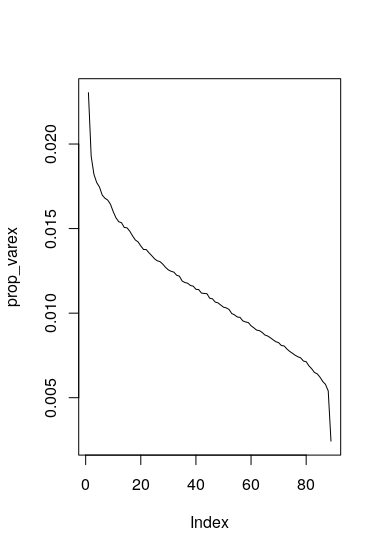
\includegraphics[width=0.60\linewidth]{../../PCA/plot/variances-ALL_rete-db.png}
	\caption{Plot della rappresentazione grafica della varianza di tutti i PC del trainset delle domande nel database.}
\end{figure}
\begin{figure}[H]
\centering
	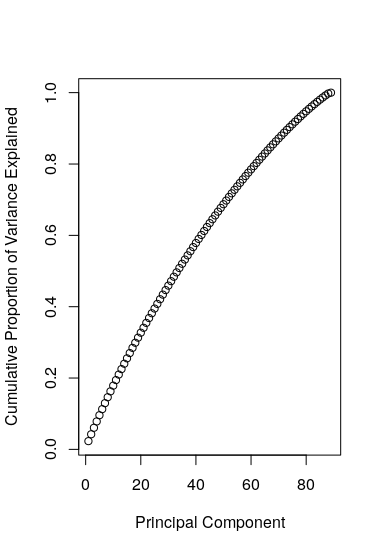
\includegraphics[width=0.60\linewidth]{../../PCA/plot/variances2-ALL_rete-db.png}
	\caption{Plot della rappresentazione grafica della varianza di tutti i PC del trainset delle domande nel database.}
\end{figure}
Non risulta sufficiente l'andamento dei plot per riuscire a definire il numero adeguato di componenti principali da utilizzare. In questi casi, \`e buona norma, fare riferimento a tre criteri:
\begin{itemize}
\item \textit{Quota della varianza totale}: si deve considerare un numero di CP tale che tenga conto di una percentuale sufficientemente elevata di varianza totale proporzionale al numero di variabili originarie (ovvero pi\`u \`e alto il numero di componenti del modello e pi\`u \`e accettata una percentuale minore di varianza spiegata).
\item \textit{Screen-graph}: fa uso dei plot degli autovalori in funzione al numero di CP. Gli autovalori sono decrescenti, per cui il grafico ha una buona possibilit\`a, di assumer\`a la forma di una spezzata con pendenza negativa.
\item \textit{Eigenvaue one o Regola di Kaiser}: afferma di considerare tutte ed esclusivamente le CP con autovalore maggiore di 1.
\end{itemize}
\noindent
Per soddisfare il \textit{primo criterio} \`e sufficiente fare riferimento a \textit{variance.percent} in get\_eigen o \textit{Proportion of Variance} in summary. Da questa asserzione ne consegue un quesito: quale \`e il numero di varianza accettabile avendo un numero di variabili molto elevato?.
Per effettuare una delle vie utilizzate \`e procedere al soddisfacimento del \textit{terzo criterio}. Gli autovalori di tutte le componenti coinvolte si possono vedere nella \textit{Standard deviation} risultante dalla summary. Le PC del modello, con autovalore superiore a 1, sono le PC contenute nell'intervallo 1-41.
Il \textit{secondo criterio}, invece, in questo caso specifico non \`e stato in grado di dirmi molto,  in quanto la diminuzione degli autovalori \`e graduale, senza salti evidenti.\\
In conclusione, ho considerato come una percentuale di copertura adeguata quella fornita dalla che 41 prime componenti principali.
\begin{figure}[H]
\centering
	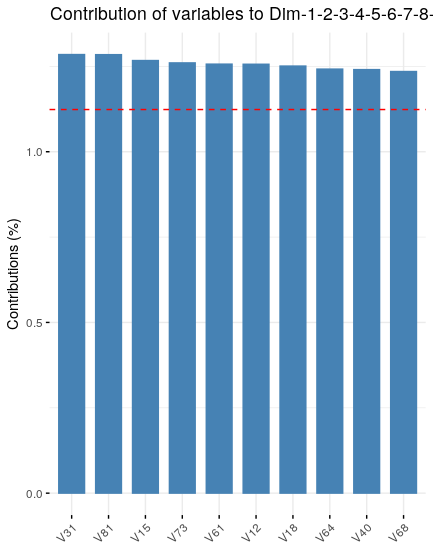
\includegraphics[width=0.60\linewidth]{../../PCA/plot/varianza-complessiva_rete-db.png}
	\caption{Rappresentazione grafica di come la varianza si distribuisce sulle PC individuate dal modello sul trainset delle domande nel database.}
\end{figure}

\subsubsection{Calcolo degli autovettori}
\label{Calcolo degli autovettori}

\begin{figure}[H]
\centering
	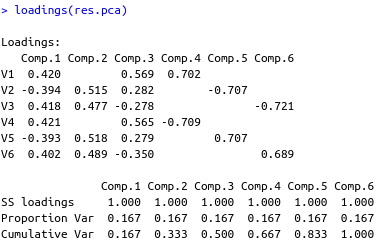
\includegraphics[width=0.60\linewidth]{../../PCA/plot/loadings_rete-prova.png}
	\caption{Autovettori del trainset di test.}
\end{figure}

\paragraph{Osservazioni}
L'analisi dei loadings sulle componenti principali permette di determinare il contributo delle variabili originarie al modello PC.\\
Per quanto riguarda l'analisi dei dati del trainset  la prima variabile ha valori  0.420, 0.569 e 0.702,  rispettivamente nelle componenti 1, 3 e 4 e sembra legarsi ai risultati nella variabile 4 (che riempie le medesime componenti oscillando di poco nei valori presentati), il medesimo match coinvolge le variabili 2 con 5 e 3 con 6.\\
Tali assunzioni sono molto pi\`u complesse da effettuare per  il trainset dei dati delle domande nel databas e  per fare ci\`o ho provveduto a calcolare la matrice correlazione.

\subsubsection{Calcolo della matrice di correlazione}
\label{Calcolo della matrice di correlazione}

\begin{figure}[H]
\centering
	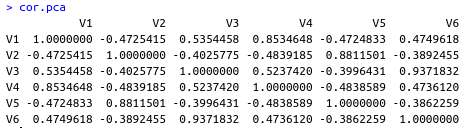
\includegraphics[width=0.60\linewidth]{../../PCA/plot/correlazione_rete-prova.png}
	\caption{Autovettori del trainset di test.}
\end{figure}

\begin{figure}[H]
\centering
	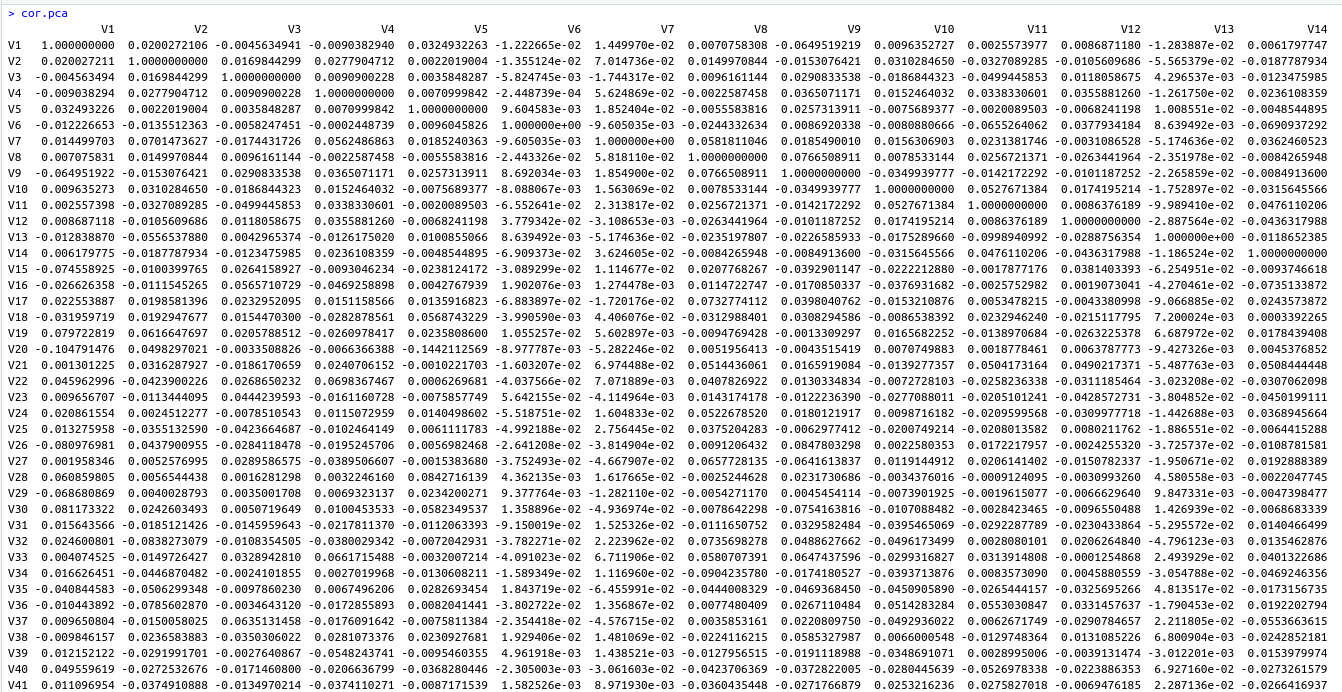
\includegraphics[width=1\linewidth]{../../PCA/plot/correlazione_rete-db.png}
	\caption{Autovettori del trainset delle domande nel database.}
\end{figure}
\noindent

I CSV generati di correlazione sono i seguenti:

\begin{figure}[H]
\centering
	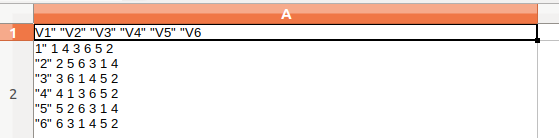
\includegraphics[width=0.60\linewidth]{../../PCA/plot/CSV_rete-prova.png}
	\caption{CSV generato a partire dalla matrice correlazione del trainset della rete.}
\end{figure}
\begin{figure}[H]
\centering
	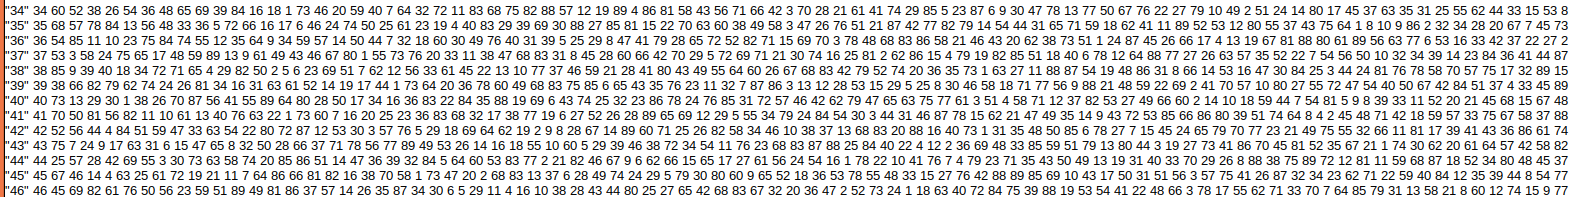
\includegraphics[width=1\linewidth]{../../PCA/plot/CSV_rete-db.png}
	\caption{CSV generato a partire dalla matrice correlazione del trainset delle domande nel database.}
\end{figure}
\noindent
I file \textit{CSV} gli ho generati prendendo la matrice correlazione, che mostra il grado di correlazione di ogni componente con ogni variabile del modello, e generandovi un data frame che mostra per ogni variabile quale \`e la componente a cui si collega in ordine decrescente (da  quella che si correla di pi\`u a quella che si correla di meno).\\ 
Da tale distribuzione dei dati, per il trainset di prova \`e apparso quello che mi aspettavo. Per esempio la variabile 1 si correla con grado massimo con se stessa, successivamente con la componente 4 (che \`e la sua domanda sorella) e successivamente con le domande 3 e 6 (i suoi genitori) e alla fine con le domande 2 e 5 (nella realt\`a queste ultime due non hanno alcuna correlazione con la domanda 1). Tale ragionamento vale per tutte le altre  5 componenti, i cui risultati rimangono coerenti con le aspettative e con ci\`o che viene dichiarato nel Grafo della conoscenza, rappresentato in §\ref{Test effettuati}.\\\\
Pensavo di poter effettuare il medesimo ragionamento anche per analisi dei dati del trainset del database, tuttavia questo non \`e stato possibile, a causa delle seguenti motivazioni:
\begin{itemize}
\item In primo luogo mi sono subito accorta che se una variabile si dichiara in correlazione con una componente, questa poi non \`e detto che sia in correlazione con la variabile;
\item Analizzando il testo delle domande, contenute nel database aziendale ho riscontrato come il modello prodotto crea relazioni strette fra domande appartenenti trivialmente a categorie diverse, (ad esempio domande che trattano relazioni con altre di serie numeriche) e meno con domande che parlano dello stesso tema.
\item Effettuando dei test nella Rete neurale costruita sul trainset delle domande nel database, non riuscivo a trovare alcun collegamento con le correlazioni che vengono evidenziata dal calcolo della PCA;
\item Il plot delle variabili mostra una vicinanza pi\`u elevata con variabili diverse rispetto a quelle indicate come quelle maggiormente correlate nella matrice di correlazione.
\end{itemize}
A questo punto ho iniziato a farmi delle domande. Escludendo un mio errore di codifica (dopo aver opportunamente effettuato un accurato controllo del codice da me prodotto) e trovandomi di fronte ad una situazione dove i risultati inerenti ai dati del trainset di prova soddisfano appieno le attese
(infatti non solo le correlazioni matchano perfettamente con quanto viene indicato dal grafo della conoscenza; ma anche il plot che viene generato dalla PCA sulle variabili presenta una coerenza stretta con tali assunzioni) ho iniziato a pensare che centrasse la possibilit\`a che ha un candidato di indovinare correttamente una risposta ad una domanda.\\\\
Ho rifatto perci\`o tutta l'analisi su un nuovo modello adoperando il trainset di prova generato da n input che tengono conto anche della possibilit\`a di indovinare. Come viene illustrato dai plots seguenti i dati individuati dal trainset di prova puro vengono totalmente falsati quando si tiene conto di tale eventualit\`a. Questo \`e il motivo per cui la \textbf{P}rincipal \textbf{C}omponent \textbf{A}nalysis non \`e in grado di dare dei risultati attendibili sul trainset delle domande del database, dove un candidato pu\`o aver risposto correttamente ad un quesito anche solo perch\`e ha "sparato a caso".

\subsection{Conclusione dell'analisi}
\label{Conclusione dell'analisi}
In conclusione quando si ha un test con domande a triplice scelta multipla un candidato ha elevata possibilit\`a di indovinare le domande che non sa e il modello creato dalla PCA con i dati delle risposte alle domande presenti nel database ne sono la prova. Questo perch\`e se la possibilit\`a di indovinare fosse bassa i risultati del modello ne verrebbero appena sporcati,  e invece invalidano completamente la possibilit\`a di avere un risultato attendibile e coerente con la realt\`a che permetta di costruire un Reticolo della Conoscenza.


\begin{figure}[H]
\centering
	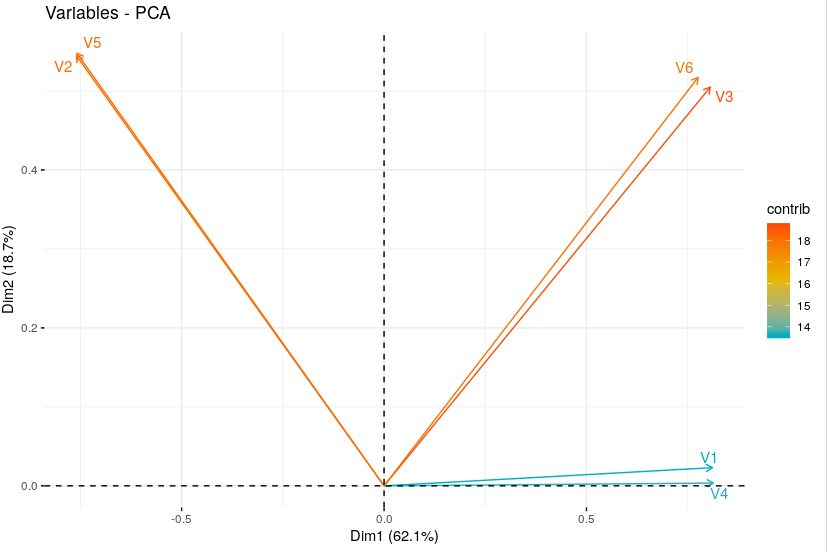
\includegraphics[width=0.80\linewidth]{../../PCA/plot/PCA.png}
	\caption{Rappresentazione per mezzo di plot di come le variabili si presentano nelle due componenti principali con il calcolo della PCA - utilizzo di trainset di prova puro sul grafo della conoscenza.}
\end{figure}
\begin{figure}[H]
\centering
	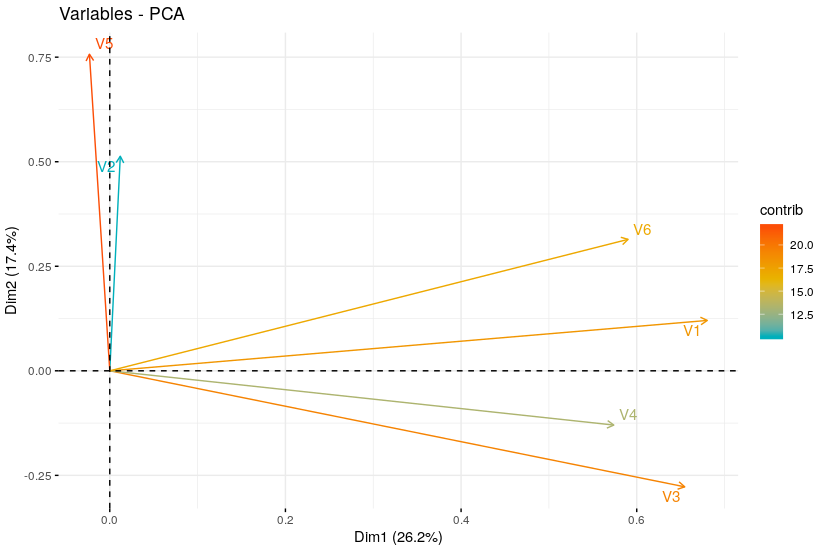
\includegraphics[width=0.80\linewidth]{../../PCA/plot/PCA-valorindovinati.png}
	\caption{Rappresentazione per mezzo di plot di come le variabili si presentano nelle due componenti principali con il calcolo della PCA - utilizzo di trainset di prova spurio con la probabilit\`a di indovinare.}
\end{figure}\pagebreak

\end{document}

